\documentclass[oneside]{report}
\usepackage[utf8]{inputenc}
\usepackage
[T5]{fontenc}
\usepackage{graphicx}
\usepackage{nameref}
\usepackage{multicol}
\usepackage{multirow}
\usepackage{algorithm}
\usepackage{algpseudocode}
\usepackage{booktabs}
\usepackage{amsthm}
\usepackage{listings}
\usepackage{spverbatim}
\usepackage[bottom]{footmisc}
\usepackage{lscape}
\usepackage{indentfirst}
%\usepackage{algorithmic}
\bibliographystyle{unsrt}

\algrenewcommand\algorithmicrequire{\textbf{Input:}}
\algrenewcommand\algorithmicensure{\textbf{Output:}}

% set font, font size and spacing
\usepackage{times}
\usepackage{scrextend}
\changefontsizes{13pt}
\renewcommand{\baselinestretch}{1.5}
% section spacing
\usepackage{titlesec}
\titlespacing*{\section}{0pt}{0.5\baselineskip}{0.2\baselineskip}
\titlespacing*{\subsection}{0pt}{0.4\baselineskip}{0.2\baselineskip}

\renewcommand{\thesection}{\thechapter.\arabic{section}}
\renewcommand{\thesubsection}{\thesection.\arabic{subsection}}
\renewcommand{\thesubsubsection}{\thesubsection.\arabic{subsubsection}}

\titleformat{\section}
  {\raggedright\fontsize{13}{16.8}\selectfont\bfseries}
  {\thesection.}{1em}{}

\titleformat{\subsection}
  {\raggedright\fontsize{13}{15.6}\selectfont\bfseries}
  {\thesubsection.}{1em}{}

\titleformat{\subsubsection}
  {\raggedright\fontsize{13}{15.6}\selectfont\bfseries}
  {\thesubsubsection.}{1em}{}

% setup page layout
\usepackage[a4paper,left=35mm,top=25mm,bottom=20mm,right=20mm,]{geometry}
\usepackage{tikz}
\usetikzlibrary{calc}
\usetikzlibrary{decorations.pathmorphing}

% Acronyms Auto
\usepackage[nopostdot,toc,acronym,nomain,nonumberlist]{glossaries}
\makeglossaries
\setacronymstyle{long-short}
\loadglsentries[acronym]{FrontMatter/Acronyms}
\setlength{\glsdescwidth}{0.7\linewidth}

% natbib
% if use natbib, please comment out the cite
% \usepackage[numbers, square, round]{natbib}

\usepackage[
    bibstyle=bwl-FU,
    backend=biber,
    doi=false,isbn=false,url=false,eprint=false,
    citestyle=ieee,
    style = numeric,
    maxcitenames=2,
    maxbibnames=3,
]{biblatex}
\addbibresource{references.bib}

% Citation
% \usepackage{cite}

% % prevent text overflow
% \usepackage{babel}
% \newcommand\fh{\babelhyphen{hard}}

% Change indent
% \usepackage{indentfirst} % indent also after section titles
\setlength{\parindent}{1cm}
\usepackage{enumitem}
\setlist{leftmargin=1cm}

% paragraph spacing
\setlength{\parskip}{0.5em}

% Change enumerate label
\usepackage{enumitem}

% Page numbering at the center top of page
% \usepackage{fancyhdr} % Custom headers and footers
% \pagestyle{fancyplain} % Makes all pages in the document conform to the custom headers and footers
% \fancyhead[L]{}% Empty left header
% \fancyhead[C]{\thepage} % Page numbering for center header  
% \fancyhead[R]{}% Empty right header
% \fancyfoot[L]{}% Empty left footer
% \fancyfoot[C]{}% Empty center footer
% \fancyfoot[R]{}% Empty left footer

\usepackage{fancyhdr}
\pagestyle{fancy}
\fancyhf{}                      % Xóa tất cả header/footer mặc định
\fancyhead[C]{\thepage}         % Số trang ở giữa header
\renewcommand{\headrulewidth}{0pt} % Bỏ đường kẻ ngang dưới header

\fancypagestyle{plain}{
    \fancyhf{}
    \fancyhead[C]{\thepage}
    \renewcommand{\headrulewidth}{0pt}
}

% Math equation
\usepackage{amssymb}
\usepackage{amsmath}

% Table
\usepackage{multirow}
\usepackage{longtable}
\usepackage{bigstrut}

% Cover
\usepackage{pdfpages}

% Subfigure
\usepackage{caption}
\usepackage{subcaption}

% pstricks fig
\usepackage{epsfig}

% Table of Contents
\usepackage[hidelinks]{hyperref}
% Uncomment if you want leading dot for chapter
\usepackage{tocloft}
\usepackage[nottoc]{tocbibind}

\renewcommand{\cftsecaftersnum}{.}
\renewcommand{\cftsubsecaftersnum}{.}
\renewcommand{\cftsubsubsecaftersnum}{.}

\makeatletter
\renewcommand{\@cftmaketoctitle}{%
  \vspace*{\cftbeforetoctitleskip}%
  \interlinepenalty\@M
  {\parindent\z@\centering\fontsize{16}{19.2}\selectfont\bfseries\contentsname\par}%
  \vspace{\cftaftertoctitleskip}%
  \par\nobreak}

\renewcommand{\@cftmakeloftitle}{%
  \vspace*{\cftbeforeloftitleskip}%
  \interlinepenalty\@M
  {\parindent\z@\centering\fontsize{16}{19.2}\selectfont\bfseries\listfigurename\par}%
  \vspace{\cftafterloftitleskip}%
  \par\nobreak}

\renewcommand{\@cftmakelottitle}{%
  \vspace*{\cftbeforelottitleskip}%
  \interlinepenalty\@M
  {\parindent\z@\centering\fontsize{16}{19.2}\selectfont\bfseries\listtablename\par}%
  \vspace{\cftafterlottitleskip}%
  \par\nobreak}
\makeatother

\setlength{\cftbeforetoctitleskip}{0pt}
\setlength{\cftaftertoctitleskip}{10pt}
\setlength{\cftbeforeloftitleskip}{0pt}
\setlength{\cftafterloftitleskip}{10pt}
\setlength{\cftbeforelottitleskip}{0pt}
\setlength{\cftafterlottitleskip}{10pt}

\renewcommand{\cftchappresnum}{CHAPTER }
\renewcommand{\cftchapaftersnum}{: }
\setlength{\cftchapnumwidth}{7em}
\renewcommand{\cftpartleader}{\cftdotfill{\cftdotsep}}
\renewcommand{\cftchapleader}{\cftdotfill{\cftdotsep}}
\renewcommand{\cftdotsep}{1.5}

%preamble auto add toc
% \usepackage{tocbibind}

\newtheorem{definition}{Definition}
\newtheorem{example}{Example}
\newtheorem{theorem}{Theorem}
\newtheorem{proposition}{Proposition}
\usepackage[export]{adjustbox}  % Put this in your preamble

% table fixed width column
\usepackage{array}
\newcolumntype{L}[1]{>{\raggedright\let\newline\\\arraybackslash\hspace{0pt}}m{#1}}
\newcolumntype{C}[1]{>{\centering\let\newline\\\arraybackslash\hspace{0pt}}m{#1}}
\newcolumntype{R}[1]{>{\raggedleft\let\newline\\\arraybackslash\hspace{0pt}}m{#1}}

\title{HaUI Thesis}
\author{Nguyen Tuan Anh}
\date{May 2026}

\makeatletter
\def\@makeschapterhead#1{%   % cho \chapter* (Abstract, ToC,...)
  {\parindent \z@ \centering
    \normalfont
    \fontsize{16}{19.2}\selectfont \bfseries #1\par\nobreak
    \vskip 10\p@
  }}
\def\@makechapterhead#1{%    % cho \chapter thường (Chapter 1, 2,...)
  {\parindent \z@ \centering \normalfont
    \fontsize{16}{19.2}\selectfont\bfseries CHAPTER \thechapter: #1\par\nobreak
    \vskip 10\p@
  }}
\makeatother

\begin{document}
%---------------------------------------------
% Front Matter
%---------------------------------------------
% \begin{titlepage}
%     \begin{tikzpicture}[overlay,remember picture]
%         \draw [line width=3pt]
%             ($ (current page.north west) + (2.0cm,-2.0cm) $)
%             rectangle
%             ($ (current page.south east) + (-1.5cm,1.8cm) $);
%         \draw [line width=1pt]
%             ($ (current page.north west) + (2.15cm,-2.15cm) $)
%             rectangle
%             ($ (current page.south east) + (-1.65cm,1.95cm) $); 
%     \end{tikzpicture}
    
%     \begin{center}
%         % \vspace*{1cm}
%         \normalsize
%         \textbf{HANOI UNIVERSITY OF INDUSTRY \\
%         SCHOOL OF INFORMATION \& COMMUNICATIONS TECHNOLOGY}

%         \vspace{1.5cm}
%         
\includegraphics[width=0.6\textwidth]{FrontMatter/sict.png}
            
%         \vspace{1.5cm}
%         \large
%         \textbf{NGUYEN TUAN ANH}
            
%         \vspace{2cm}
%         \large
%         \textbf{OPTIMIZING A CASCADED DEEP LEARNING ARCHITECTURE FOR VIETNAMESE TEXT RECOGNITION SYSTEM FROM IMAGES USING RT-DETR AND PARSeq\\}   
%         \vspace{3cm}
%         \large
%         \textbf{BACHELOR THESIS \\
%         Major}: Information Technology       

%         \vspace{1cm}
%         \textbf{Supervisor: Assoc. Prof. Dr. Nguyen Thi Kim Son} 
        
%         \vfill
%         \large
%         \textbf{HA NOI - 2026}
%     \end{center}
% \end{titlepage}

\begin{titlepage}
    \begin{tikzpicture}[overlay,remember picture]
        \draw [line width=3pt]
            ($ (current page.north west) + (2.0cm,-2.0cm) $)
            rectangle
            ($ (current page.south east) + (-1.5cm,1.8cm) $);
        \draw [line width=1pt]
            ($ (current page.north west) + (2.15cm,-2.15cm) $)
            rectangle
            ($ (current page.south east) + (-1.65cm,1.95cm) $); 
    \end{tikzpicture}
    
    \begin{center}
        \vspace*{-1.5cm}
        \large
        \textbf{MINISTRY OF INDUSTRY AND TRADE \\
        HANOI UNIVERSITY OF INDUSTRY}

        \vspace{-1em}
        % \vspace{0.3cm}
        \noindent\rule{0.4\textwidth}{0.4pt}
        \vspace{0.3cm}

        % \vspace{1cm}
        
\includegraphics[width=0.3\textwidth]{FrontMatter/logo_haui.png}
        
        \vspace{0.5cm}

        \large
        GRADUATION THESIS \\
        MAJOR: INFORMATION TECHNOLOGY
        
        \vspace{1.0cm}
        
        \large
        \textbf{OPTIMIZING A CASCADED DEEP LEARNING ARCHITECTURE FOR VIETNAMESE TEXT RECOGNITION SYSTEM FROM IMAGES USING RT-DETR AND PARSEQ}
            
        \vspace{2.5cm}
        
        % \normalsize
        \begin{tabular}{l l l}
            \textbf{Supervisor}   & \textbf{:} & \textbf{Assoc. Prof. Dr. Nguyen Thi Kim Son} \\[6pt]
            \textbf{Student}      & \textbf{:} & \textbf{Nguyen Tuan Anh} \\[6pt]
            \textbf{Student's ID} & \textbf{:} & \textbf{2022602757} \\
        \end{tabular}
            
        \vfill
        \large
        Hanoi - 2026
    \end{center}
\end{titlepage}

\pagenumbering{roman}
\setcounter{page}{1}
% \chapter
*{Declaration}
\addcontentsline{toc}{chapter}{Declaration}

I declare that I am the sole author of this thesis and that it has not been previously submitted for any other academic or professional qualification. I confirm that the work submitted results from my efforts, supplemented by the valuable guidance and support of Assoc. Prof. Dr. Nguyen Thi Kim Son, for the main purpose of graduation.

All information, data, and results included in this thesis are original and have not been plagiarized from any other sources. All references used in this thesis are duly cited and listed in the reference section.

I take full responsibility for the content and integrity of this thesis, under the regulations of the HaUI School of Information & Communications Technology.
\\
\\
\\
\\
\\
\begin{table}[!ht]
\begin{tabular}{p{0.7\textwidth}c}
 & Ha Noi, 2026 \\
 & Student \\
 &              \\
 &              \\
 &              \\
 & \textbf{Nguyen Tuan Anh} 
\end{tabular}
\end{table}
% \chapter*{Supervisor’s Approval}

\addcontentsline{toc}{chapter}{Supervisor’s Approval}

”I hereby approve that the thesis is accepted in its present form for committee evaluation as part of the requirements for the Bachelor’s Degree in Information Technology at the School of Information & Communications Technology.”
\\
\\
\\
\\
\\
\begin{table}[!ht]
\begin{tabular}{p{0.7\textwidth}c}
 & Ha Noi, 2026 \\
 & Supervisor \\
 &              \\
 &              \\
 &              \\
 & \textbf{Nguyen Thi Kim Son} 
\end{tabular}
\end{table}
% \include{FrontMatter/Publications}
\chapter*{Acknowledgements}

\addcontentsline{toc}{chapter}{Acknowledgements}

I wish to convey my profound appreciation to my esteemed mentor, Assoc. Prof. Dr. Nguyen Thi Kim Son, whose unwavering assistance and sagacious counsel have been instrumental throughout my scholarly pursuits. Her tutelage has markedly enriched my intellectual growth, and I am at a loss to adequately express the depth of my gratitude for his encouragement and erudition. The privilege of working under her aegis at the School of Information \& Communications Technology - Hanoi University of Industry has been an extraordinary experience. I am deeply honored to have benefited from her tutelage and will forever treasure the wisdom and personal development I have attained under her assiduous guidance.

I am also immensely grateful to the School of Information \& Communications Technology, HaUI, for fostering an environment that is both nurturing and intellectually stimulating, thereby enabling students to flourish. The institution's commitment to equity and professionalism in its pedagogical ethos has been a cornerstone of my educational journey. I extend my heartfelt thanks to all the educators and instructors whose profound knowledge and unwavering dedication have made an indelible impact. Their fervor for pedagogy and readiness to mentor students have been pivotal in enhancing my comprehension, as well as that of my peers, of the intricacies of computer science.

I wish to express my sincere and heartfelt gratitude to my cherished friends for their unwavering and heartfelt companionship and support. During dark and trying moments of adversity and despondency, they have stood as an unyielding and steadfast bulwark, offering not merely their presence but also deeply empathetic and attentive listening, profound and genuine understanding, and wise and thoughtful advice. Their encouragement has shone as a radiant and uplifting beacon of hope, enabling me to persevere through the most daunting and challenging of times.

Finally, to my beloved and treasured family, I extend my deepest and most fervent gratitude for your infinite and unconditional love, steadfast and unwavering support, and the countless and selfless sacrifices you have made on my behalf. Your unshakable and inspiring faith in my abilities has imbued my endeavors with profound and enduring meaning and has served as the powerful and relentless driving force behind my every hard-earned achievement. Your presence has been a constant and unwavering source of fortitude, wisdom, and gentle guidance, and I am profoundly and eternally thankful for the absolutely indispensable and pivotal role you have played in my extraordinary and transformative academic odyssey.

% \chapter*{Abstract}
\addcontentsline{toc}{chapter}{Abstract}

The digitization of Vietnamese documents has become an urgent priority for administrative agencies and enterprises. Optical character recognition (OCR) serves as the key enabling technology, yet the orthographic complexity of Vietnamese, which superimposes multiple layers of vowel modifications and tonal diacritics onto a Latin-derived base script, poses substantial challenges. General-purpose OCR systems struggle because Vietnamese requires a vast character inventory, visual distinctions between diacritically similar characters are often minimal under realistic conditions, and existing systems fail to handle diverse layouts and arbitrary text orientations caused by page skew or document curvature.

This thesis proposes a cascaded deep learning architecture that addresses these challenges through two independently optimized stages. The first stage employs a fine-tuned RT-DETR V2 detector extended with an auxiliary angle regression head, which predicts text line orientations using sine-cosine parameterization and is trained with Gaussian Wasserstein Distance loss to provide geometrically unified supervision over oriented bounding boxes. The second stage uses a fine-tuned PARSeq Vision Transformer recognizer adapted to Vietnamese via vocabulary extension to approximately 310 composite tokens, class-weighted cross-entropy loss to counteract severe character frequency imbalance, and a phonological validity mask applied at decoding time. A perspective-corrected inter-stage interface converts arbitrarily oriented text regions into upright rectangular crops, ensuring that angular localization quality directly benefits diacritical recognition accuracy.

To address data scarcity, two large-scale synthetic generation pipelines are developed. The detection pipeline produces approximately 130,000 annotated document images spanning seven layout archetypes with uniform angular coverage across the full $[0^\circ, 360^\circ)$ rotation range. The recognition pipeline produces approximately 2,000,000 labeled text line crops via a three-branch parallel strategy covering clean printed, augmented scene text, and mixed-background conditions.

Experimental evaluation demonstrates that the proposed system substantially outperforms established baselines. On detection, the fine-tuned RT-DETR model achieves F1@0.50 of 0.501 and mAP@0.5:0.95 of 0.147, compared to 0.134 and 0.008 for EAST. On recognition, PARSeq achieves a Character Error Rate of 10.18\% and Word Error Rate of 34.71\%, outperforming VietOCR, PaddleOCR, Tesseract, and EasyOCR. The complete system is deployed as a modular pipeline producing structured transcripts, with component encapsulation facilitating future upgrades without full retraining.

\vspace{-0.5cm}
\begin{flushleft}
    \textit{\textbf{Keywords:} Vietnamese OCR, Text Detection, Text Recognition, Oriented Bounding Box, RT-DETR, PARSeq, Gaussian Wasserstein Distance, Synthetic Data Generation, Deep Learning.}
\end{flushleft}
\changefontsizes[16pt]{13pt}

% \chapter*{Tóm tắt}
\addcontentsline{toc}{chapter}{Tóm tắt}
Số hóa tài liệu tiếng Việt đã trở thành ưu tiên cấp thiết đối với các cơ quan hành chính và doanh nghiệp. Nhận dạng ký tự quang học (OCR) là công nghệ then chốt, tuy nhiên chữ viết tiếng Việt đặt ra nhiều thách thức, bao gồm kho ký tự khổng lồ, khác biệt thị giác nhỏ giữa các ký tự có dấu phụ tương đồng, cùng bố cục đa dạng và hướng văn bản tùy ý.

Đồ án này đề xuất một kiến trúc học sâu theo tầng gồm hai giai đoạn được tối ưu hóa độc lập. Giai đoạn đầu sử dụng RT-DETR V2 được tinh chỉnh với đầu hồi quy góc bằng tham số hóa sine-cosine và hàm mất mát Gaussian Wasserstein Distance. Giai đoạn hai sử dụng PARSeq Vision Transformer được tinh chỉnh cho tiếng Việt bằng cách mở rộng bộ từ vựng lên khoảng 310 token tổ hợp, hàm mất mát cross-entropy có trọng số theo lớp, và mặt nạ kiểm tra tính hợp lệ âm vị tại bước giải mã. Một bộ xử lý trung gian hiệu chỉnh phối cảnh chuyển đổi vùng văn bản nghiêng thành ảnh cắt thẳng đứng, liên kết chất lượng định vị góc với độ chính xác nhận dạng dấu phụ.

Để giải quyết khan hiếm dữ liệu, hai pipeline tổng hợp độc lập được xây dựng: pipeline phát hiện tạo ra khoảng 130.000 ảnh tài liệu có chú thích trên bảy kiểu bố cục với phạm vi góc đầy đủ $[0^\circ, 360^\circ)$, và pipeline nhận dạng tạo ra khoảng 2.000.000 ảnh cắt có nhãn trên ba điều kiện gồm văn bản in sạch, văn bản cảnh tăng cường, và nền hỗn hợp.

Thực nghiệm cho thấy hệ thống đề xuất vượt trội đáng kể so với các baseline. RT-DETR đạt F1@0.50 là 0,501 và mAP@0.5:0.95 là 0,147, so với 0,134 và 0,008 của EAST. PARSeq đạt Tỷ lệ lỗi ký tự 10,18\% và Tỷ lệ lỗi từ 34,71\%, vượt trội so với VietOCR, PaddleOCR, Tesseract và EasyOCR. Hệ thống được triển khai dưới dạng pipeline mô-đun với đóng gói thành phần giúp thuận tiện nâng cấp mà không cần huấn luyện lại toàn bộ.
\vspace{-0.5cm}
\begin{flushleft}
    \textit{\textbf{Từ khóa:} OCR tiếng Việt, Phát hiện văn bản, Nhận dạng văn bản, Hộp giới hạn có hướng, RT-DETR, PARSeq, Gaussian Wasserstein Distance, Tổng hợp dữ liệu, Học sâu.}
\end{flushleft}
\changefontsizes[16pt]{13pt}


% Show ToC and change title to Table of Contents
\setcounter{secnumdepth}{3}
\renewcommand{\contentsname}{TABLE OF CONTENTS}
{\renewcommand{\baselinestretch}{1.2}\normalsize
\tableofcontents}

% Show Acronyms and add it to ToC
\printglossary[title={LIST OF ABBREVIATION},type=acronym,style=long]
\clearpage

% Show list of 
\renewcommand{\listfigurename}{LIST OF FIGURES}
\listoffigures
\clearpage
\renewcommand{\listtablename}{LIST OF TABLES}
\listoftables
\clearpage

% \chapter*{Abstract}
\addcontentsline{toc}{chapter}{Abstract}

The digitization of Vietnamese documents has become an urgent priority for administrative agencies and enterprises. Optical character recognition (OCR) serves as the key enabling technology, yet the orthographic complexity of Vietnamese, which superimposes multiple layers of vowel modifications and tonal diacritics onto a Latin-derived base script, poses substantial challenges. General-purpose OCR systems struggle because Vietnamese requires a vast character inventory, visual distinctions between diacritically similar characters are often minimal under realistic conditions, and existing systems fail to handle diverse layouts and arbitrary text orientations caused by page skew or document curvature.

This thesis proposes a cascaded deep learning architecture that addresses these challenges through two independently optimized stages. The first stage employs a fine-tuned RT-DETR V2 detector extended with an auxiliary angle regression head, which predicts text line orientations using sine-cosine parameterization and is trained with Gaussian Wasserstein Distance loss to provide geometrically unified supervision over oriented bounding boxes. The second stage uses a fine-tuned PARSeq Vision Transformer recognizer adapted to Vietnamese via vocabulary extension to approximately 310 composite tokens, class-weighted cross-entropy loss to counteract severe character frequency imbalance, and a phonological validity mask applied at decoding time. A perspective-corrected inter-stage interface converts arbitrarily oriented text regions into upright rectangular crops, ensuring that angular localization quality directly benefits diacritical recognition accuracy.

To address data scarcity, two large-scale synthetic generation pipelines are developed. The detection pipeline produces approximately 130,000 annotated document images spanning seven layout archetypes with uniform angular coverage across the full $[0^\circ, 360^\circ)$ rotation range. The recognition pipeline produces approximately 2,000,000 labeled text line crops via a three-branch parallel strategy covering clean printed, augmented scene text, and mixed-background conditions.

Experimental evaluation demonstrates that the proposed system substantially outperforms established baselines. On detection, the fine-tuned RT-DETR model achieves F1@0.50 of 0.501 and mAP@0.5:0.95 of 0.147, compared to 0.134 and 0.008 for EAST. On recognition, PARSeq achieves a Character Error Rate of 10.18\% and Word Error Rate of 34.71\%, outperforming VietOCR, PaddleOCR, Tesseract, and EasyOCR. The complete system is deployed as a modular pipeline producing structured transcripts, with component encapsulation facilitating future upgrades without full retraining.

\vspace{-0.5cm}
\begin{flushleft}
    \textit{\textbf{Keywords:} Vietnamese OCR, Text Detection, Text Recognition, Oriented Bounding Box, RT-DETR, PARSeq, Gaussian Wasserstein Distance, Synthetic Data Generation, Deep Learning.}
\end{flushleft}
\changefontsizes[16pt]{13pt}


%--------------------------------------------- 
% Main content
%---------------------------------------------
\pagenumbering{arabic}
\setcounter{page}{1}
\chapter{Introduction}

\section{Motivation}

\subsection{Digitizing Vietnamese Documents}

Vietnam has undergone rapid administrative modernization over the past two decades, driven by government-led digital transformation initiatives that aim to replace manual, paper-based workflows with electronic document management systems across public and private sectors \cite{Decision749QDTTg_2020}. This transition affects an extraordinarily broad range of document types: tax invoices, procurement records, official correspondence, land registration certificates, health records, educational transcripts, court decisions, and legislative texts, all of which are currently stored in paper form in archives accumulated over many decades of governance \cite{MST_Egov_Strategy_2021}. The sheer volume of existing paper documentation, combined with the ongoing generation of new paper records in agencies that have not yet completed their digital transitions, creates a pressing demand for automated document digitization at scale \cite{Kaiser2022}.

OCR serves as the key enabling technology for this digitization effort. Without OCR, scanned documents remain image files that cannot be searched, indexed, or used as inputs to downstream information extraction systems. With OCR, scanned documents become machine-readable text that can be ingested into databases, processed by information retrieval pipelines, and made accessible through full-text search interfaces. The economic and administrative value of this transformation is substantial: automated OCR processing can reduce manual data entry costs by orders of magnitude, accelerate document retrieval times from hours to milliseconds, and enable the construction of queryable national archives that would otherwise require prohibitive amounts of human labor to maintain \cite{Palm2017}.

The digitization of Vietnamese historical and archival documents carries significant cultural and scholarly value. Libraries, museums, and academic institutions hold large collections of historical Vietnamese texts, newspaper archives, colonial-era administrative records, and literary manuscripts that are deteriorating due to age and environmental factors. Digitization through OCR preserves these documents in a form that can be archived, replicated, and made accessible to researchers and the public worldwide. The linguistic and historical content of such archives is irreplaceable once lost, giving OCR development for Vietnamese a preservation dimension that extends beyond immediate administrative utility.

The educational sector similarly benefits from large-scale OCR capability. Textbooks, examination records, student transcripts, and pedagogical materials exist predominantly in printed form across Vietnamese educational institutions, and their digitization enables new forms of accessibility, translation, and adaptive learning that are impossible with image-only storage. The combination of administrative, archival, and educational demand establishes a compelling and multi-dimensional motivation for investing in high-quality Vietnamese OCR technology.

\subsection{Challenges in Vietnamese OCR}

Vietnamese presents a unique set of challenges for optical character recognition that extend well beyond those encountered in most Latin-script languages and that are not adequately addressed by general-purpose OCR systems developed without Vietnamese-specific adaptation \cite{Le2025}. These challenges arise from two interconnected sources: the exceptional orthographic complexity of the Vietnamese writing system, and the limited availability of annotated data resources for training and evaluating recognition models in this language \cite{Le2025}.

At the orthographic level, Vietnamese employs a diacritical system of unusual density and lexical significance. Unlike most Latin-script languages where diacritical marks play a limited and relatively predictable role, Vietnamese superimposes two independent layers of diacritical modification onto its base characters simultaneously. The first layer consists of vowel quality markers that alter the phonetic identity of the base vowel, producing three distinct characters from the base vowel \textit{a} (plain \textit{a}, circumflex \textit{a}, and breve \textit{a}), with analogous modifications applying to several other base vowels and yielding seventeen distinct vowel surface forms in total \cite{Nguyen2012}. The second layer consists of tonal markers encoding one of six lexically contrastive tones through five diacritical marks and the absence of any mark for the level tone. Because these two layers of modification can co-occur on a single character, the resulting Vietnamese character inventory is several times larger than that of unaccented Latin-script languages, posing a direct challenge to recognition models trained on standard Latin benchmarks \cite{Nguyen2021}.

From the perspective of OCR model design, this orthographic complexity produces two primary failure modes. The first is character-level confusion, in which visually similar composite glyphs are misclassified due to the small spatial extent of distinguishing diacritical strokes relative to the base character body. At low image resolutions or under degraded scan conditions, the difference between a dot below and a hook above, or between a circumflex and a breve, can be reduced to a handful of pixels, falling below the discriminative capacity of feature extractors that were not specifically trained on Vietnamese text \cite{Nguyen2021}. The second failure mode is segmentation ambiguity, in which the spatial extent of a composite Vietnamese character overlaps with neighboring characters or with the ascender and descender zones of adjacent text lines, causing detection-based systems to either merge distinct characters or fragment a single character across multiple detected regions \cite{Nguyen2021}.

Beyond orthographic complexity, the diversity of Vietnamese document formats introduces additional technical challenges for both detection and recognition stages. Vietnamese administrative documents span a wide range of layouts, including single-column official correspondence, multi-column legal texts, tabular financial records, receipts with characteristic formatting structures, and identity documents with fixed field templates. Real-world documents may be captured through flatbed scanning, camera photography, or mobile phone imaging, each introducing different geometric distortions, illumination conditions, and resolution characteristics. Text lines in scanned documents are frequently not perfectly horizontal due to page skew introduced during scanning, and documents with physical curvature produce locally varying text orientations that challenge axis-aligned detection systems. The diversity of Vietnamese font styles across formal administrative typefaces, commercial display fonts, and historical typographic conventions further expands the distribution that a robust OCR system must cover.

A compounding challenge is the limited availability of annotated Vietnamese OCR datasets suitable for training modern deep learning systems. Compared to the rich benchmark ecosystems surrounding English and Chinese OCR, Vietnamese-specific datasets remain sparse in terms of scale, annotation granularity, and document type diversity \cite{Nguyen2021}. The most linguistically diverse publicly available Vietnamese OCR benchmark, VinText \cite{Nguyen2021}, comprises approximately 2,000 real images, which is several orders of magnitude smaller than the large-scale multilingual datasets used to train state-of-the-art multilingual OCR systems such as MLT \cite{Nayef2017}. The absence of character-level annotations in most Vietnamese datasets further restricts the ability to train and evaluate detection components at fine granularity, and the lack of standardized evaluation protocols across existing datasets makes cross-study comparison unreliable.

The scarcity of annotated data is directly exacerbated by the orthographic complexity of Vietnamese: annotating Vietnamese text requires annotators who can reliably distinguish between visually similar tone-diacritic combinations, which demands higher annotator skill and more careful quality control than annotation of unaccented Latin text. This creates a self-reinforcing bottleneck in which the language most in need of specialized OCR systems is also the most difficult to annotate efficiently, limiting the scale of training data that can be produced for a given annotation budget.

\subsection{The Importance of Accurate Text Recognition in Vietnamese}

The importance of recognition accuracy in Vietnamese OCR systems is not merely a matter of benchmark performance but is directly tied to the practical consequences of recognition errors in the deployment contexts where these systems are most needed. Vietnamese is a tonal language in which diacritical marks carry lexical meaning: altering or omitting a single diacritical mark on a character does not produce a misspelling of the intended word but an entirely different word with a potentially unrelated meaning \cite{Le2025}. For example, the syllables \textit{ma}, \textit{mà}, \textit{má}, \textit{mả}, \textit{mã}, and \textit{mạ} (differing only in tonal mark) denote distinct words corresponding to ghost, but, cheek, tomb, horse and rice seedling respectively \cite{Nguyen2019}. A recognition error that substitutes one tonal mark for another therefore does not corrupt a character; it changes the identity of the word, and the corrupted output may be another valid Vietnamese word that passes any lexical validity check without revealing the underlying error \cite{Pham2017}.

This property of Vietnamese orthography makes recognition errors both more consequential and harder to detect than in most other Latin-script languages. In the context of administrative document processing, recognition errors on invoice fields, contract terms, official names, or legal identifiers can introduce downstream errors that propagate through automated extraction pipelines without triggering any alert. The consequences range from financial discrepancies in automated invoice processing to legal ambiguities in digitized contract records and identity mismatches in administrative databases \cite{Park2019}. Vietnamese government agencies processing tax invoices, procurement records, and official correspondence through OCR-based digitization pipelines are particularly exposed to these risks, as the orthographic complexity of Vietnamese text imposes additional demands on the recognition component and recognition errors on diacritical marks can produce semantically distinct output that corrupts downstream information extraction \cite{Huang2019}.

In historical archive digitization, the stakes are different but equally high. OCR errors in the transcription of historical documents create persistent inaccuracies that, once introduced into searchable archives, are difficult to identify and correct without reviewing the original scanned images. A digitized historical corpus with significant recognition error rates is not merely imperfect but may be actively misleading, attributing incorrect words or names to historical figures and creating artifacts in computational analyses that rely on the corpus as primary data. The cultural and scholarly value of accurate historical transcription makes recognition accuracy a prerequisite for the usefulness of any archival OCR system, not simply a performance optimization.

In information retrieval systems, recognition accuracy directly determines recall, the fraction of relevant documents retrieved in response to a query. If the OCR output for a document contains character errors, keyword searches for terms that appear in that document may fail to retrieve it, effectively making the document invisible to the information retrieval system. Given that Vietnamese administrative archives contain documents that may be retrieved for legal, historical, or policy purposes years or decades after their creation, the long-term consequences of recognition errors that suppress relevant retrieval are substantial. High recognition accuracy is therefore not a quality-of-life improvement but a functional requirement for OCR-based information retrieval to serve its intended purpose.

These considerations collectively establish that Vietnamese OCR is a problem of practical importance that demands solutions commensurate with the difficulty of the language and the stakes of the deployment context. The remainder of this thesis is dedicated to developing and evaluating such a solution.

\subsection{Recent Applications in Document OCR}

The practical relevance of optical character recognition extends well beyond academic benchmarks, with deployed OCR systems now underpinning a wide range of real-world document processing workflows across industries and public institutions. The maturation of deep learning-based detection and recognition architectures has enabled OCR to move from controlled laboratory settings into operational environments characterized by document diversity, scale requirements, and strict accuracy demands. This section surveys three representative application domains that illustrate the breadth of contemporary OCR deployment: administrative and financial document processing, identity document recognition, and historical archive transcription. Each domain presents a distinct set of technical challenges that contextualize the practical value of the Vietnamese OCR system developed in this thesis.

\subsubsection{Administrative and Financial Document Processing}
The digitization of administrative and financial documents, including invoices, receipts, purchase orders, and tax forms, represents one of the most commercially mature applications of OCR technology. Organizations processing large volumes of such documents have strong economic incentives to automate extraction of structured information such as vendor names, dates, line items, and totals, reducing reliance on manual data entry and accelerating downstream business processes. Early OCR-based approaches to this problem relied on template matching against fixed document layouts, but the diversity of invoice formats across vendors and jurisdictions made template-based systems brittle and expensive to maintain \cite{Palm2017}.

More recent work has framed invoice and receipt understanding as a joint OCR and information extraction problem, in which text detection and recognition are coupled with named entity recognition and document layout analysis to produce structured output from unstructured document images. The CORD dataset \cite{Park2019} and the SROIE benchmark \cite{Huang2019} established standardized evaluation frameworks for receipt OCR and key information extraction, driving the development of end-to-end trainable systems that simultaneously localize text, transcribe it, and classify it into semantic categories. LayoutLM \cite{Xu2020} extended transformer-based language models to the document understanding domain by incorporating two-dimensional positional embeddings that encode the spatial coordinates of each text token alongside its semantic embedding, enabling the model to exploit document layout structure as an additional signal for information extraction. Subsequent iterations including LayoutLMv2 \cite{Xu2022} and LayoutLMv3 \cite{Huang2022} further integrated visual features from document images directly into the pretraining objective, producing unified multimodal representations that have become the dominant paradigm for structured document understanding

The relevance of this application domain to Vietnamese OCR is direct. Vietnamese government agencies and enterprises generate large volumes of administrative documents including tax invoices, procurement records, and official correspondence, all of which are candidates for automated digitization. The orthographic complexity of Vietnamese text imposes additional demands on the OCR component of such pipelines, as recognition errors on diacritical marks can produce semantically distinct output that corrupts downstream information extraction.

\subsubsection{Identity Document Recognition}
Identity document recognition, encompassing the automated extraction of personal information from national identity cards, passports, driving licenses, and similar credentials, constitutes another high-value OCR application domain with stringent accuracy and reliability requirements. Errors in recognized identity fields can have serious consequences in contexts such as border control, financial onboarding, and voter registration, making this one of the most demanding real-world OCR deployment scenarios.

Early systems exploited the structured layouts of standardized identity documents, using template registration to locate predefined field regions before applying OCR within each. Machine-readable zones (MRZ) provided a constrained recognition target well-suited to classical techniques, given their limited character set and fixed typography. However, the diversity of identity document formats across countries and the presence of security printing features, holographic overlays, and variable background textures have motivated the adoption of deep learning-based approaches that generalize across document types without requiring per-format template engineering. The MIDV-500 dataset \cite{Bulatov2019} established a standardized benchmark for identity document analysis by providing annotated samples across 50 document types from different countries under varied capture conditions including flat, curved, and perspective-distorted document images, enabling more rigorous evaluation of generalizable identity document recognition systems.

More recent work has framed identity document recognition as an end-to-end structured information extraction problem, combining text detection, recognition, and field classification within a unified pipeline \cite{Tran2019}. Rather than treating each processing stage independently, these systems jointly optimize detection and recognition objectives, enabling the model to leverage layout structure as a supervisory signal for improving transcription accuracy across variable document formats. For Vietnamese identity documents specifically, the transition from the old nine-digit citizen identification card to the new twelve-digit CCCD format introduced new layout conventions and font specifications that required OCR systems to be retrained or fine-tuned, highlighting the importance of adaptable recognition architectures \cite{Nguyen2022}. The cascaded detection-recognition design adopted in this thesis is well suited to this setting, as the modular architecture allows the detection and recognition components to be independently fine-tuned when document specifications change.

Across both application domains surveyed in this section, a consistent pattern emerges: the performance of deployed OCR systems is ultimately bounded by the quality of the underlying text detection and recognition components, and improvements to these core components translate directly into downstream application quality. This observation reinforces the motivation for the thesis at hand, which targets the detection and recognition pipeline as the primary locus of improvement for Vietnamese document OCR.

\subsection{Vietnamese-Specific OCR Challenges and Solutions}
Vietnamese presents a unique set of challenges for optical character recognition that extend well beyond those encountered in most Latin-script languages, and that are not adequately addressed by OCR systems designed for general multilingual use. While the deep learning architectures surveyed in the preceding section have demonstrated strong performance across a broad range of scripts and document types, their direct application to Vietnamese text without domain-specific adaptation consistently yields suboptimal results. These shortcomings stem from two interconnected factors that distinguish Vietnamese OCR from the general case.

The first factor is linguistic and orthographic in nature. Vietnamese employs a diacritical system of exceptional complexity, in which multiple combining marks can co-occur on a single character to encode both vowel quality and lexical tone simultaneously. This orthographic density produces a character inventory significantly larger than that of unaccented Latin-script languages, and introduces visual ambiguities that challenge both detection and recognition components of an OCR pipeline. The second factor is resource-related. Despite growing interest in Vietnamese document digitization, the landscape of publicly available annotated datasets and standardized benchmarks for Vietnamese OCR remains considerably less developed than the corresponding ecosystems for English, Chinese, or Arabic, constraining the training and rigorous evaluation of recognition models.

These two factors are closely interrelated: the orthographic complexity of Vietnamese makes the annotation process more demanding and error-prone, which in turn limits the scale and coverage of available datasets, which in turn impedes the development of models robust enough to handle the full range of Vietnamese diacritical variation. This section examines both dimensions in turn, first analyzing the specific diacritical and tonal characteristics of Vietnamese that create difficulties for OCR models, and then surveying the existing datasets and benchmarks that have been developed to support Vietnamese text recognition research, identifying the gaps that motivate the data preparation strategy adopted in this thesis.

\subsubsection{Diacritical Marks and Tonal Complexity}
\label{sec:diacritical_marks_and_tonal_complexity}
Vietnamese presents a distinctively challenging target for optical character recognition due to its orthographic system, which overlays multiple layers of diacritical modification onto a Latin-derived base script. Unlike most Latin-script languages, where diacritics serve a limited and relatively predictable role, Vietnamese employs diacritics at two independent levels simultaneously: vowel quality markers that alter the phonetic identity of the base character, and tonal markers that specify one of six lexically contrastive tones \cite{Nguyen2012}. These two layers of modification can co-occur on a single character, producing composite glyphs that are visually dense and spatially compact, creating significant difficulties for both text detection and recognition systems.

At the level of vowel modification, Vietnamese augments several base vowels with diacritic strokes that fundamentally change their phonetic identity. The vowel \textit{a}, for instance, yields three distinct characters: \textit{a}, \textit{a with circumflex} (â), and \textit{a with breve} (ă), each representing a different phoneme and therefore a different lexical unit. Similar modification patterns apply to the vowels \textit{e}, \textit{o}, and \textit{u}, yielding a total of seventeen distinct vowel surface forms from seven base vowels. When tonal markers are superimposed on these modified vowels, the resulting character set expands substantially. Vietnamese defines six tones encoded through five diacritical marks, namely the grave, acute, hook above, tilde, and dot below, plus the absence of any tone mark for the level tone. Combining all vowel modifications with all tonal possibilities yields a Vietnamese character inventory that is several times larger than that of unaccented Latin-script languages, posing a direct challenge to recognition models trained on standard Latin benchmarks \cite{Nguyen2021}.

From the perspective of OCR model design, this orthographic complexity manifests in two principal failure modes. The first is character-level confusion, where visually similar composite glyphs are misclassified as one another due to the small spatial extent of distinguishing diacritical strokes relative to the base character body. At low image resolutions or under degraded scan conditions, the difference between a dot below and a hook above, or between a circumflex and a breve, can be reduced to a handful of pixels, well below the discriminative capacity of feature extractors trained on higher-resolution data \cite{Nguyen2021}. The second failure mode is segmentation ambiguity, where the spatial extent of a composite Vietnamese character overlaps with neighboring characters or with the ascender and descender zones of adjacent text lines, causing segmentation-based detectors to either merge distinct characters or fragment a single character across multiple segments \cite{Nguyen2021}. This segmentation problem is particularly acute in printed documents with tight inter-line spacing and diverse font styles, which fall squarely within the scope of this thesis.

Existing approaches to mitigating these challenges fall into two broad categories. The first encompasses character set redesign strategies, in which the model output vocabulary is explicitly constructed to include all valid Vietnamese composite characters as atomic units, rather than decomposing them into base characters and combining diacritics \cite{Nguyen2021}. This atomic treatment forces the recognition model to learn a direct mapping from visual glyph to full Unicode character, avoiding the error accumulation that arises when base character and diacritic predictions are made independently. The second category leverages linguistic constraints through language model integration, exploiting the fact that not all combinations of base character and diacritical marks are phonologically valid in Vietnamese, and that valid tone-vowel combinations follow predictable phonotactic rules that can be encoded as decoding constraints \cite{Nguyen2021}. The methodology adopted in this thesis draws on both categories, as detailed in Chapter \ref{chapter:methodology_chapter3}.

\subsubsection{Existing Vietnamese OCR Datasets and Benchmark}
\label{sec:existing_vnese_ocr_datasets_and_benchmark}

The availability of high-quality annotated datasets is a prerequisite for training and evaluating robust Vietnamese OCR systems, yet the Vietnamese OCR research community has historically been constrained by a limited and fragmented landscape of publicly available corpora. Compared to the rich benchmark ecosystems surrounding English and Chinese OCR, Vietnamese-specific datasets remain sparse in terms of both scale and diversity, a gap that has directly impeded the development of generalizable recognition models \cite{Nguyen2021}.

Among the earliest publicly available resources is the VOHTR2018 dataset \cite{Nguyen2018}, which targets offline handwritten Vietnamese text and provides word-level and line-level images annotated with ground truth transcriptions. While valuable for handwriting recognition research, VOHTR2018 does not address the printed document domain and its annotation granularity is insufficient for training text detection models that require bounding box supervision at the word or character level. Its annotations also do not generalize readily to scene text conditions, limiting its utility for the broader Vietnamese OCR task.

A more recent and comprehensive contribution is VinText \cite{Nguyen2021}, a Vietnamese scene text dataset comprising over 2,000 real images collected from diverse real-world environments including street signs, storefronts, menus, and printed documents. VinText provides word-level polygon annotations along with full transcriptions and constitutes the most linguistically diverse publicly available Vietnamese OCR benchmark to date. Its inclusion of natural scene images with complex backgrounds, arbitrary text orientations, and mixed font styles makes it substantially more challenging than synthetic corpora and more representative of deployment conditions. A key contribution of VinText is its dictionary-guided recognition framework, which explicitly incorporates Vietnamese lexical constraints to resolve diacritical ambiguities at inference time \cite{Nguyen2021}. However, its scale remains modest relative to large-scale multilingual benchmarks such as MLT \cite{Nayef2017} and LSVT \cite{Sun2019}, and its coverage of formal administrative document layouts is limited.

Across these datasets, several consistent gaps are apparent. First, no existing Vietnamese OCR benchmark provides sufficient coverage of the full range of document types encountered in administrative digitization workflows, including low-resolution scans, faded ink, and degraded print quality. Second, character-level annotation remains rare, with most datasets providing only word-level or line-level ground truth, which limits the ability to train and evaluate detection components at finer granularity. Third, the absence of a standardized evaluation protocol across datasets makes cross-paper comparison of reported results unreliable. These gaps collectively motivate the data preparation strategy adopted in this work, which combines synthetic generation with domain-specific augmentation to compensate for the scarcity of real annotated Vietnamese document images, as described in Chapter \ref{chapter:methodology_chapter3}.

\section{Proposed Approach: Deep Learning-Based \\ Vietnamese OCR}

\subsection{Approach}
\label{sec:approach_1_2_1}
The approach adopted in this thesis is grounded in the observation that the two fundamental subtasks of document OCR, spatial localization of text regions and sequential transcription of their contents, have distinct computational requirements that are best addressed by architectures specifically optimized for each. Rather than pursuing a single end-to-end model that attempts to solve both problems simultaneously within a shared representation, this work proposes a cascaded two-stage architecture in which a specialized detector and a specialized recognizer are independently trained and then connected through a well-defined geometric interface.

For the detection stage, this thesis adopts RT-DETR V2 \cite{Zhao2024}, a real-time transformer-based object detector that combines the spatial feature extraction efficiency of convolutional networks with the global context modeling capacity of transformer self-attention. RT-DETR is selected over convolutional alternatives such as EAST \cite{Zhou2017} and CRAFT \cite{Baek2019} for several reasons that are directly relevant to the Vietnamese document setting. Its anchor-free, set-prediction formulation eliminates the need to manually engineer aspect ratio priors for Vietnamese text lines, which vary considerably across document types and orientations. Its hybrid encoder captures both local character-level texture and global line-level structure within a single forward pass, without the receptive field limitations inherent to purely convolutional architectures. Furthermore, its strong out-of-the-box localization accuracy on general object detection benchmarks provides a favorable initialization for domain-specific fine-tuning on Vietnamese text data. To enable oriented bounding box prediction, which is necessary for tightly enclosing skewed and rotated text lines encountered in real Vietnamese documents, RT-DETR V2 is extended with an auxiliary angle regression head that produces sine-cosine angle predictions, coupled with a Gaussian Wasserstein Distance (GWD) loss \cite{Yang2022} that provides geometrically principled supervision over all five oriented box parameters jointly.

For the recognition stage, this thesis adopts PARSeq \cite{Bautista2022}, a Vision Transformer-based scene text recognizer that formulates character sequence prediction as a permutation language modeling problem. PARSeq is selected because its ViT encoder captures the fine-grained spatial detail required to distinguish Vietnamese diacritical marks that differ only by subtle stroke variations, while its permutation-trained decoder implicitly learns a bidirectional language model that can resolve character-level ambiguities using both preceding and following character context. This bidirectional reasoning capability is particularly valuable for Vietnamese, where the distinction between visually similar tone-diacritic combinations is frequently underdetermined by local visual evidence alone and requires contextual inference from the surrounding character sequence. PARSeq is adapted to the Vietnamese domain through a carefully designed vocabulary extension that treats each composite Vietnamese glyph as an atomic output token, class-weighted training that compensates for the severe frequency imbalance between common and rare diacritical combinations, and a phonological validity mask applied at decoding time to suppress linguistically impossible character outputs.

The combination of these two components into a cascaded pipeline represents the central technical contribution of this thesis. The modular design allows each component to be independently trained, evaluated, and improved without requiring full system retraining, which is a practical necessity given the limited availability of annotated Vietnamese OCR data. The interface between the two stages performs perspective-corrected cropping using the oriented bounding box predictions from the detector, converting arbitrarily rotated text line regions into upright rectangular crops before passing them to the recognizer. This cropping strategy is not merely an engineering convenience but is a direct operationalization of the theoretical argument that tight angular localization in the detection stage is a prerequisite for accurate diacritical recognition in the transcription stage.

\subsection{Pipeline Components and Workflow}

The end-to-end pipeline transforms a raw input document image into a structured collection of recognized text strings through five sequential processing stages, each implemented as an independent module with well-defined input and output interfaces.

The pipeline transforms a raw input document image into a structured collection of recognized text strings through five sequential stages: image ingestion and preprocessing, oriented text line detection, bounding box post-processing, perspective-corrected cropping, and character sequence recognition. Each stage is implemented as an independent module, enabling the system to be executed as a unified inference pipeline. The mechanics of each stage, including intermediate tensor shapes and inter-stage data contracts, are elaborated in Chapter~\ref{chapter:methodology_chapter3}.

\subsection{Model Optimization Strategy}

Achieving competitive performance on Vietnamese text with the proposed cascaded architecture requires targeted optimization of both pipeline components, since the general-purpose pretrained checkpoints for RT-DETR and PARSeq were not trained on Vietnamese document data and do not natively support the full Vietnamese composite character set. The optimization strategy applied to each stage is briefly summarized here; complete technical details are provided in Chapter 3.

For the detection stage, the primary optimization challenge is adapting a model pretrained on general object detection to the single-class task of Vietnamese text line localization with oriented bounding box output. This is addressed through a combination of domain-specific synthetic data generation and a carefully staged fine-tuning protocol. The synthetic data pipeline produces approximately 130,000 annotated document images spanning seven layout archetypes, including single-column administrative correspondence, multi-column texts, receipt formats, and fully rotated scatter layouts, with exact oriented bounding box annotations derived analytically from rendering parameters. A critical engineering contribution of this pipeline is the correction of an angle distribution collapse in the base generator, which ensures that the training set provides uniform angular coverage across the full $[0^\circ, 360^\circ)$ rotation range. The fine-tuning protocol employs a three-tier differential learning rate schedule that assigns distinct learning rates to the pretrained backbone, the transformer encoder-decoder, and the newly initialized angle regression head, combined with metric-driven progressive backbone unfreezing to protect pretrained representations during early training. The loss function combines standard detection losses with a cosine angle loss and the GWD loss weighted at $\lambda_{\text{gwd}} = 3.0$, reflecting the importance of angular supervision for downstream recognition quality.

For the recognition stage, the primary optimization challenges are vocabulary expansion and class imbalance. The standard PARSeq vocabulary of 94 printable ASCII characters is insufficient to represent the full Vietnamese composite character set, which requires approximately 232 additional atomic tokens covering all phonologically valid combinations of vowel modification diacritics and tonal markers. The vocabulary is extended by replacing the output projection layer with a new linear layer initialized from pretrained weights for shared characters and from random values for new Vietnamese glyphs, allowing the model to retain its pretrained decoding capability for Latin characters while learning the new Vietnamese distributions through fine-tuning. Class-weighted cross-entropy loss is applied to counteract the severe frequency imbalance between common unaccented characters and rare tone-diacritic combinations that are disproportionately critical for lexical correctness. Fine-tuning is conducted on a 2,000,000-image synthetic recognition corpus generated by a three-branch parallel pipeline covering clean printed, augmented scene text, and mixed-background conditions. At inference time, a phonological validity mask restricts decoder outputs to phonologically possible Vietnamese character sequences, reducing the rate of linguistically impossible predictions under degraded image conditions. Together, these adaptations produce a recognition model that outperforms all evaluated baselines on the Vietnamese test set, including systems specifically designed for Vietnamese such as VietOCR \cite{QuocBinhNguyen2020}.

\section{Objectives, Outline and Scope}

\subsection{Research Objectives}

This thesis pursues three concrete and measurable research objectives, each targeting a distinct bottleneck in the Vietnamese document OCR pipeline.

The first objective is to develop an oriented text line detector capable of accurately localizing Vietnamese text lines across a wide range of document layouts and text orientations, with tight bounding box fitting sufficient to minimize background noise and character truncation in the crops delivered to the recognition stage. This objective is operationalized through the extension of RT-DETR V2 with a sine-cosine angle regression head and GWD loss, and through the development of a synthetic detection training corpus with uniform angular coverage.

The second objective is to develop a Vietnamese text recognition model that achieves competitive character and word accuracy across the full inventory of Vietnamese composite characters, including rare tone-diacritic combinations that are systematically underrepresented in general-purpose scene text recognition training data. This objective is operationalized through vocabulary extension, class-weighted training, phonological validity constraints, and fine-tuning on a large-scale Vietnamese-specific synthetic recognition corpus.

The third objective is to integrate the detection and recognition components into a unified, modular end-to-end pipeline with a perspective-corrected inter-stage interface, and to evaluate the integrated system against established detection and recognition baselines on held-out Vietnamese document test sets. This objective provides the empirical validation that grounds the architectural and methodological claims of the thesis.

\subsection{Scope}

The scope of this work is delimited along three dimensions. With respect to text modality, the system is designed and evaluated exclusively for printed Vietnamese text in formal and semi-formal document contexts, including administrative correspondence, financial records, receipts, and identity documents. Handwritten Vietnamese text falls outside the scope of the current system, as it presents additional challenges from variable stroke widths and unconstrained character forms that are not addressed by the training data or model architectures adopted here. With respect to language, the system is optimized specifically for Vietnamese and is evaluated only on Vietnamese text, though the cascaded architecture is language-agnostic and could in principle be extended to other languages with complex diacritical systems through corpus and vocabulary substitution. With respect to evaluation data, the detection and recognition components are each evaluated on held-out synthetic test sets derived from the same generation pipelines used for training, and the characterization of any residual domain gap relative to real scanned documents is based on qualitative analysis and is identified as a primary direction for future work.

\subsection{Thesis Outline}

To systematically address the aforementioned objectives, this thesis is organized into five chapters as follows.

\textbf{Chapter 1: Introduction} establishes the motivation for the work, surveys the demand for Vietnamese document digitization, characterizes the technical challenges that distinguish Vietnamese OCR from the general case, and introduces the proposed cascaded approach alongside the research objectives and scope.

\textbf{Chapter 2: Related Works} surveys four areas of prior research that inform the proposed system: traditional OCR methods and their limitations, deep learning approaches to text detection and recognition with particular focus on the RT-DETR and PARSeq architectures, Vietnamese-specific OCR challenges arising from diacritical complexity and data scarcity, and representative real-world OCR application domains that contextualize the practical value of the system.

\textbf{Chapter 3: Methodology and Implementation} presents the complete technical design of the proposed system, covering the cascaded architecture and end-to-end pipeline design, the synthetic data generation pipelines for both detection and recognition stages, the model optimization strategies including the angle head design and GWD loss configuration for RT-DETR and the vocabulary extension and linguistic constraints for PARSeq, and the system integration connecting both components through the perspective-corrected inter-stage interface.

\textbf{Chapter 4: Experiments} reports the experimental evaluation, including the experimental setup, the selected detection and recognition baselines, quantitative results on the Vietnamese document test sets, and a discussion of the results, identified limitations, and concrete directions for future improvement.

\textbf{Chapter 5: Conclusions} summarizes the principal technical contributions of the thesis, reflects on how the proposed system addresses the challenges identified in this introduction, draws conclusions from the experimental findings, and outlines the practical value of the system for Vietnamese document digitization workflows.

\setcounter{chapter}{0}
\chapter{Related Works}

\section{Traditional Optical Character Recognition Methods}

Traditional Optical Character Recognition (OCR) methods, developed primarily before the advent of modern machine learning and deep learning techniques, rely heavily on rule-based, template-based, or heuristic-driven approaches to transform text from images into machine-readable formats. These methods leverage image processing techniques, handcrafted feature extraction, and predefined geometric patterns to recognize characters, often with a focus on digitized scanned documents. While foundational to the field of automated text recognition, these approaches are characterized by their dependence on manual effort and domain-specific expertise, which limits their scalability and adaptability in complex visual environments. This section reviews the key paradigms in traditional OCR, traces their evolution over time, and highlights their contributions and shortcomings.

\subsection{Template Matching and Early Approaches}

One of the earliest notable efforts in traditional OCR is the work of Mori, Suen, and Yamamoto \cite{Mori1992}, who synthesized and developed first-generation OCR techniques. The approach during this period utilized basic image processing to perform template matching, comparing images pixel-by-pixel against a predefined library of character templates. While straightforward and computationally efficient for uniform, typewritten documents, this method was highly sensitive to variations in font style, size, and image quality, making the system brittle when confronted with diverse document conditions.

Lenet and colleagues later pioneered the application of convolutional neural network precursors combined with traditional sliding-window classifiers for digit recognition \cite{LeCun1998}. This hybrid approach improved upon purely template-based systems by incorporating learned local features, but still required carefully engineered preprocessing pipelines and struggled to generalize beyond constrained digit vocabularies. Casey and Lecolinet \cite{Casey1996} further systematized recognition strategies through a taxonomy of structural decomposition approaches, in which characters are broken into primitive strokes and reassembled via graph-matching algorithms. This approach excelled in domain-specific contexts such as postal code recognition, but its reliance on a fixed set of structural primitives restricted flexibility when confronted with diverse font families, as adapting the system to new scripts required redesigning the primitive library from scratch.

\subsection{Structural and Feature-Based Methods}

The OCR field advanced considerably with research on structural and topological feature extraction, exemplified by the work of Tappert et al. \cite{Tappert1990}. Rather than relying on pixel-level comparison, this approach extracted key geometric characteristics from text, such as loops, lines, and stroke intersections, to serve as inputs to classification algorithms. This strategy proved particularly valuable for processing standardized printed documents, where character geometry is well-defined and consistent. However, it required significant manual tuning to design features robust to noise and font variation, highlighting the heavy dependence of traditional methods on human intervention and domain knowledge.

Nagy \cite{Nagy2000} extended this paradigm by exploring document layout analysis as a precursor to character recognition. The proposed system uses geometric segmentation to identify text blocks, columns, and lines before passing individual regions to a character classifier, marking a step forward in handling multi-column documents. Its dependence on clean binarization and rigid layout assumptions, however, limited robustness across varied real-world document conditions, where uneven illumination, physical page curvature, and background clutter frequently violate the assumptions required for reliable segmentation.

\subsection{Statistical and Sequence-Based Methods}

A significant conceptual advance came with the application of Hidden Markov Models (HMMs) to text recognition, as demonstrated in works such as those by Anigbogu \cite{Anigbogu1995}. Rather than treating each character as an isolated unit, HMM-based systems model text as a sequence of observations derived from sliding vertical windows across a text line, allowing recognition to proceed without explicit character segmentation. This formulation was groundbreaking because it enabled the recognition of cursive scripts and noisy text in which individual character boundaries are ambiguous. The effectiveness of HMM-based systems, however, depended heavily on the quality of manually crafted sliding-window features and the accompanying statistical language model, limiting their transferability across scripts and document types.

\subsection{Traditional Vietnamese OCR}

Researchers further expanded the scope of OCR by addressing highly complex writing systems, with Vietnamese receiving specific attention due to its dense diacritical structure \cite{Le2025}. Traditional approaches to Vietnamese OCR typically combined rule-based projection profiles to separate main characters from tonal marks, followed by heuristic scoring methods to reassociate diacritics with their base characters. This pipeline exploited the relatively predictable vertical arrangement of Vietnamese composite glyphs in printed documents, where tone marks appear consistently above or below the base vowel region.

While functional for clean, high-resolution administrative documents, these methods struggled to scale across varied background noise conditions and failed almost entirely on scene text images captured in natural environments. The projection-profile assumption breaks down when text lines are skewed, when characters overlap due to tight tracking, or when tonal marks are partially obscured, all of which are common in real-world Vietnamese document collections. The fragility of this approach under these conditions directly motivated the adoption of data-driven recognition methods capable of learning robust representations of Vietnamese composite glyphs without hand-engineered segmentation rules.

\subsection{Strengths and Limitations}

Traditional OCR methods possess notable strengths in controlled settings. Their rule-based and template-driven design ensures predictable, interpretable outputs well-suited to digitizing typewritten administrative records or standardized printed forms. They perform reliably on uniform, high-resolution documents with consistent fonts and layouts, and require minimal labeled data and computational resources compared to modern deep learning systems, making them appropriate for early digitization efforts or resource-limited environments.

Their limitations, however, are fundamental rather than incidental. Handcrafted features and rigid templates severely restrict scalability and adaptability across diverse document types. HMM-based systems are brittle under varying noise conditions due to their dependence on manually crafted features. Perhaps most critically, traditional methods lack the capacity to model contextual dependencies across characters or words, producing recognition outputs that are locally plausible but globally inconsistent, a particularly serious limitation for morphologically complex scripts such as Vietnamese in which diacritical context determines word identity. These shortcomings collectively drove the transition toward automated, data-driven approaches, which are examined in the following section.

\section{Deep Learning Approaches for OCR}

Deep learning has fundamentally transformed Optical Character Recognition, shifting the paradigm from handcrafted feature engineering to end-to-end trainable neural architectures. Unlike traditional methods, deep learning-based OCR systems generalize across diverse scripts, fonts, and document conditions with significantly reduced reliance on domain-specific heuristics. This section surveys the major methodologies driving state-of-the-art OCR performance, tracing the progression from early convolutional approaches to modern transformer-based systems.

The foundations of deep learning in OCR were established through CNNs as feature extractors for text detection \cite{LeCun1998}. EAST proposed a direct regression pipeline predicting word-level bounding boxes in a single forward pass. CRAFT extended this by modeling character-level affinity, enabling detection of curved text, while DBNet introduced differentiable binarization to learn the detection threshold adaptively. On the recognition side, the CRNN combined CNNs with RNNs via CTC loss for direct text-line transcription without character segmentation. Attention-based models such as ASTER improved on CTC by incorporating spatial rectification, and ABINet introduced explicit bidirectional language modeling in parallel with visual decoding. Most recently, transformer architectures yielded models such as PARSeq and RT-DETR, which achieve state-of-the-art accuracy at real-time speed. Collectively, these advances reflect the replacement of modular pipelines with unified, data-driven architectures.

\subsection{CNN-based Text Detection}

CNNs enabled text detection systems to localize text regions with far greater robustness than traditional methods by learning hierarchical features directly from data. Three landmark architectures — EAST, CRAFT, and DBNet — illustrate the evolution from single-shot regression to flexible segmentation-driven approaches.

EAST marked a departure from multi-stage pipelines by proposing a fully convolutional, single-shot architecture predicting text regions at the pixel level \cite{Zhou2017}. A feature pyramid network aggregates multi-scale features, which feed two output branches: a score map for text presence and a regression branch for bounding box geometry and rotation. This streamlined design enables real-time inference on benchmarks such as ICDAR 2015 \cite{Karatzas2015}. Its primary limitation is confinement to rotated rectangles, making it unsuitable for curved or arbitrarily shaped text; performance also degrades on densely packed regions.

CRAFT addressed these limitations by shifting detection granularity to the character level \cite{Baek2019}. Rather than predicting bounding boxes directly, it produces two heat maps: a region score for character centers and an affinity score for spatial relationships between adjacent characters. Post-processing groups characters by affinity to recover text instances of arbitrary shape. A notable challenge is the absence of character-level annotations in most datasets, which the authors address via weakly supervised training with pseudo ground truth from a pretrained detector — a strategy that introduces noise and inconsistencies at character boundaries.

DBNet introduced adaptive binarization directly into the segmentation pipeline \cite{Liao2019}. Traditional approaches apply a fixed threshold to probability maps in a step decoupled from training; DBNet instead parameterizes binarization as a differentiable operation with a learned threshold map, enabling joint end-to-end optimization. This yields sharper text boundaries and better separation of closely spaced text instances, achieving strong results on curved-text benchmarks Total-Text and CTW1500. Its remaining limitation is a post-processing step requiring connected component analysis with sensitive hyperparameters.

While EAST, CRAFT, and DBNet represent substantial advances, they share a common constraint: their convolutional inductive bias limits the receptive field and makes modeling long-range spatial dependencies difficult, motivating the shift to transformer-based architectures.

\subsection{Transformer-based Text Detection and RT-DETR}

The self-attention mechanism at the core of transformers \cite{Vaswani2023} allows each position in a feature map to attend globally to all other positions, which is valuable for text detection where distant contextual cues inform local decisions. DETR \cite{Carion2020} reformulated object detection as a direct set prediction problem, removing hand-designed anchors and non-maximum suppression through bipartite matching at training time. Despite competitive accuracy, its slow convergence and insufficient inference speed limited practical deployment. Deformable DETR \cite{Zhu2021} addressed convergence by replacing dense attention with deformable attention attending to a sparse set of learned reference points, reducing complexity from quadratic to linear. DAB-DETR and DN-DETR further improved training stability, yet transformer detectors continued to lag behind CNNs in inference speed.

RT-DETR \cite{Zhao2024} resolved this bottleneck through a hybrid architecture combining convolutional efficiency with transformer expressiveness. As shown in Figure \ref{fig:rtdetr_architecture}, it consists of three components: a convolutional backbone, a hybrid encoder, and a transformer decoder with IoU-aware query selection. A pretrained backbone (e.g., ResNet) extracts multi-scale feature maps encoding both texture and semantic information.

\begin{figure}[H]
\centering
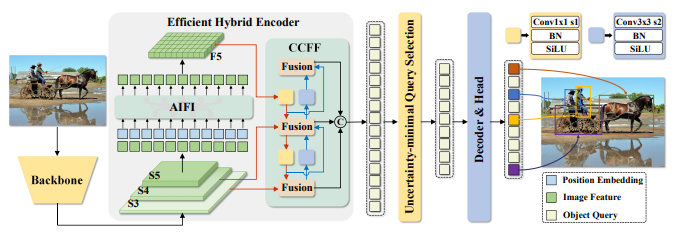
\includegraphics[width=0.8\linewidth]{images/rtdetr_architecture.png}
\caption[Overview of RT-DETR]{\textit{Overview of RT-DETR \cite{Zhao2024}}}
\label{fig:rtdetr_architecture}
\end{figure}

The hybrid encoder is RT-DETR's central innovation as illustrated in Figure \ref{fig:rtdetr_hybrid_encoder}. The Attention-based Intra-scale Feature Interaction (AIFI) module applies transformer self-attention exclusively to the highest-level feature map, where low spatial resolution makes global attention computationally feasible. The CNN-based Cross-scale Feature Fusion (CCFM) module then propagates enriched semantic context to higher-resolution maps via lightweight convolutions. This design achieves a favorable balance between representational power and inference efficiency.

\begin{figure}[ht]
\centering
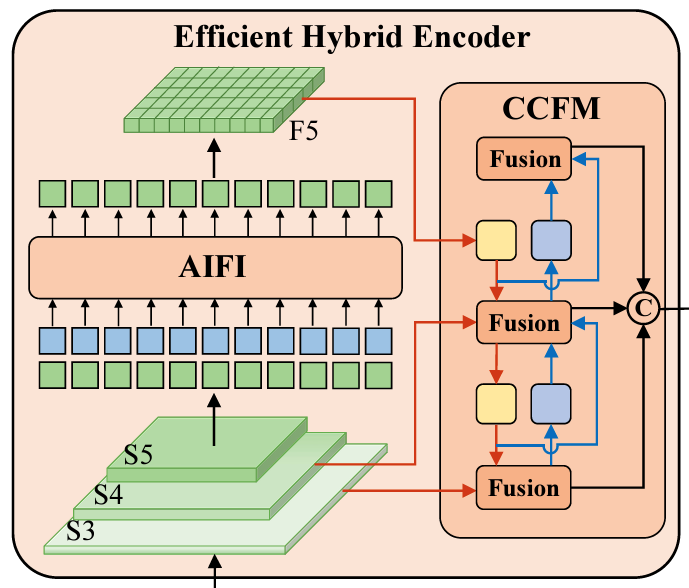
\includegraphics[width=0.6\linewidth]{images/rtdetr_hybrid_encoder.png}
\caption[Hybrid encoder of the RT-DETR model]{\textit{Hybrid encoder of the RT-DETR model \cite{Zhao2024}}}
\label{fig:rtdetr_hybrid_encoder}
\end{figure}

Query initialization is addressed through IoU-aware query selection: decoder queries are initialized from the top-scoring encoder features ranked jointly by classification confidence and predicted IoU. This yields better-calibrated initial queries than classification-only ranking, particularly for objects with high localization quality but moderate classification confidence — a common scenario in text detection.

As shown in Figure \ref{fig:rtdetr_performance}, RT-DETR with a ResNet-50 backbone achieves 53.1 AP at 108 FPS on a T4 GPU, outperforming YOLOv8-l by 1.0 AP at comparable speed. Its anchor-free design, hybrid encoder, and strong localization performance make it well-suited for Vietnamese text detection, where text lines vary considerably across document types.

\begin{figure}[ht]
\centering
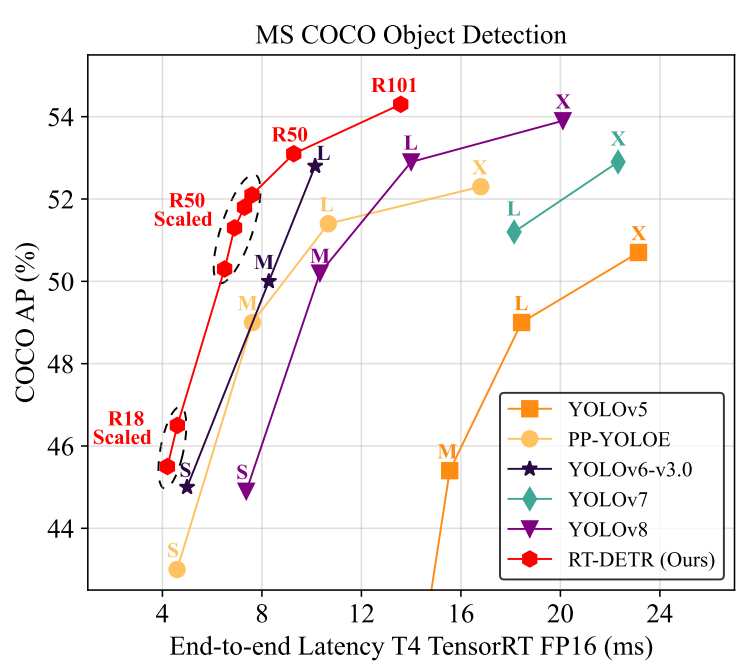
\includegraphics[width=0.6\linewidth]{images/rtdetr_performance.png}
\caption[RT-DETR latency comparison with several YOLO models]{\textit{RT-DETR latency comparison with several YOLO models \cite{Zhao2024}}}
\label{fig:rtdetr_performance}
\end{figure}

\subsection{Sequence-to-Sequence Models for Text Recognition}

Text recognition requires transcribing character sequences from images, presenting different challenges from detection. Early deep learning approaches drew from speech recognition, where recurrent architectures and probabilistic alignment had matured.

CRNN established the foundational architecture by combining a CNN feature extractor with a bidirectional LSTM, decoding output sequences via CTC loss without explicit character segmentation \cite{Shi2015}. Its simplicity and efficiency made it a widely adopted baseline. However, its recurrent bottleneck limits parallelization, and CTC's conditional independence assumption prevents explicit linguistic context modeling.

ASTER addressed geometric distortions by incorporating a learnable spatial transformer as a rectification frontend, warping the input to an approximately horizontal layout before an attention-based decoder \cite{Shi2019}. This improved accuracy on curved benchmarks such as SVT-Perspective, though the rectification adds overhead and degrades on severely distorted inputs. Attention-based encoder-decoder models more generally replaced fixed context vectors with soft alignment mechanisms, enabling selective attention to spatially relevant regions at each decoding step. AON explored multi-directional reading for irregular text, while SAR applied two-dimensional attention directly to 2D feature maps, benefiting characters with vertically complex structures.

ABINet achieved a significant conceptual advance by decoupling visual and linguistic modeling into two parallel branches \cite{Fang2021}. The visual model produces an initial prediction from image features; a separately trained bidirectional language model iteratively refines it using surrounding character context. This demonstrated that explicit linguistic modeling — rather than implicit recurrent context — is critical for high-accuracy recognition. The trade-off is added complexity from the separate language model and a more involved training process.

The progression from CRNN to ABINet reflects consistent movement toward richer contextual modeling, from local CTC decoding through soft attention to bidirectional language modeling, setting the stage for fully transformer-based recognizers.

\subsection{PARSeq and Permutation-based Recognition}

\label{sec:parseq_and_permutation_based_recognition}
PARSeq addresses limitations of prior architectures — fixed decoding orders and separately trained language models — through a unified framework combining a ViT encoder with permutation-based language modeling \cite{Bautista2022}.
The ViT encoder \cite{Dosovitskiy2021} divides the input image into a fixed grid of patches, projects each into a high-dimensional embedding, and processes all patches jointly through transformer self-attention layers. Unlike CNN encoders that aggregate context through local convolutions, the ViT captures global image structure from the first layer, relating distant character regions without deep stacking.

\begin{figure}[ht]
\centering
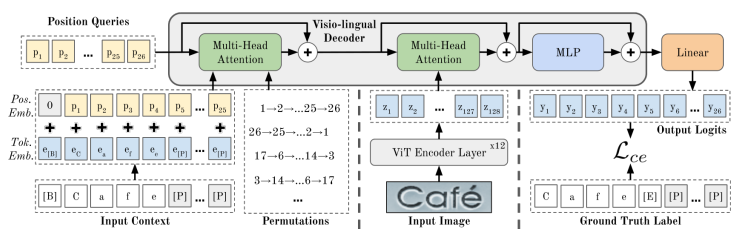
\includegraphics[width=0.8\linewidth]{images/parseq_architecture.png}
\caption[Overview of PARSeq]{\textit{Overview of PARSeq \cite{Bautista2022}}}
\label{fig:parseq_architecture}
\end{figure}

PARSeq's central innovation is its permutation-based training strategy. Rather than training the decoder in a fixed left-to-right order, PARSeq samples multiple permutations of the output sequence during training, optimizing the model to predict each character given all characters preceding it in the sampled order. This trains a single decoder to internalize all factorizations of the joint sequence probability, implicitly learning a bidirectional language model without a separate pretrained component. At inference time, an initial left-to-right pass produces a candidate sequence, which serves as context for a refinement pass correcting characters using both preceding and following context (Figure \ref{fig:parseq_permutation}). This is particularly valuable for languages with dense diacritical marks such as Vietnamese.

\begin{figure}[ht]
\centering
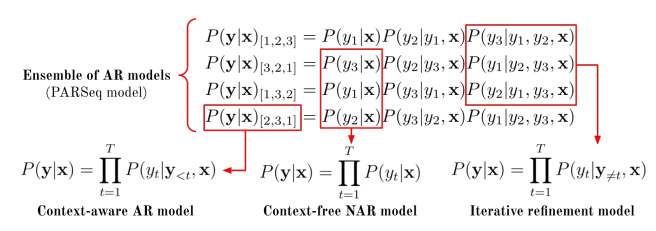
\includegraphics[width=0.8\linewidth]{images/parseq_permutation.png}
\caption[Permutation-based training strategy of PARSeq]{\textit{Permutation-based training strategy of PARSeq \cite{Bautista2022}}}
\label{fig:parseq_permutation}
\end{figure}

A further advantage is support for both autoregressive and non-autoregressive decoding within the same model, controlled by the decoder attention mask \cite{Bautista2022}. This allows practitioners to trade accuracy against speed at deployment time without retraining.

PARSeq achieved state-of-the-art accuracy across standard benchmarks (IIIT5K, SVT, ICDAR 2013/2015, SVTP, CUTE80) with a smaller parameter count than ABINet, demonstrating that permutation-based training is a more parameter-efficient mechanism for linguistic context than maintaining a separate language model. Its ViT encoder captures fine-grained spatial detail to distinguish Vietnamese diacritical marks, while its permutation-trained decoder resolves visually ambiguous characters under image degradation.

\subsection{Oriented Text Detection and Rotation-Aware Loss Functions}
\label{sec:oriented_text_detection_and_rotation_aware_loss_functions_2_2_5}

\subsubsection{Oriented Bounding Box Detection for Scene Text}
The problem of detecting arbitrarily oriented text has been an active research direction since the limitations of axis-aligned detectors became apparent on real-world scene text benchmarks. Early work on oriented text detection adapted region proposal networks to generate rotated candidate regions by augmenting the anchor parameterization with a discrete set of orientation bins. RRPN (Rotation Region Proposal Networks) \cite{Ma2018} extended the Faster RCNN framework by introducing rotation-aware anchors spanning multiple orientations and an RoI rotation pooling operation that extracts features from arbitrarily rotated candidate regions. This enabled the detector to localize text at angles not representable by axis-aligned anchors, achieving substantially improved recall on benchmarks containing multi-oriented text such as ICDAR 2015 \cite{Karatzas2015}. However, RRPN's reliance on a discrete set of predefined rotation anchors limited its angular resolution and required careful anchor design to cover the expected range of text orientations in the target domain.

TextBoxes++ \cite{Liao2018} approached the problem from a single-shot detection perspective, extending the SSD framework with irregular convolutional filters and output layers that directly regress rotated quadrilateral bounding boxes rather than axis-aligned rectangles. By predicting four corner offsets relative to a default box anchor, TextBoxes++ could represent not only rotated rectangles but also general quadrilaterals, enabling accurate enclosure of perspective-distorted text instances. This direct regression formulation avoided the angular discretization problem of anchor-based approaches but introduced training instability arising from the discontinuous nature of angular regression targets near boundary angles.

More recent work has integrated oriented detection capabilities into transformer-based frameworks, which are better suited to the anchor-free, set-prediction paradigm adopted in this thesis. Oriented RCNN \cite{Xie2021} demonstrated that a simple modification to the region proposal head, replacing axis-aligned box regression with five-parameter oriented box regression, sufficed to achieve state-of-the-art oriented detection performance without requiring specialized rotation-aware pooling operations. In the context of this work, RT-DETR is extended with an additional angle prediction head that regresses orientation as a two-dimensional unit vector in sine-cosine space, rather than as a scalar angle in degrees. This sine-cosine encoding avoids the angular discontinuity problem that arises when scalar angle regression crosses the boundary between 0 and 360 degrees, ensuring smooth and continuous gradient flow during training regardless of the predicted orientation.

\subsubsection{Gaussian Wasserstein Distance Loss for Oriented Box Regression}

A key challenge in training oriented detectors is designing a regression loss that accurately measures geometric discrepancy between predicted and ground truth OBBs. Standard IoU losses are computationally expensive and numerically unstable for rotated boxes, and yield zero gradient for non-overlapping boxes regardless of spatial proximity \cite{Yang2022}.

Yang et al. \cite{Yang2022} proposed the Gaussian Wasserstein Distance (GWD) loss by representing each oriented box as a 2D Gaussian distribution (Figure \ref{fig:gwd_gaussian}). An OBB with center $(\mu_x, \mu_y)$, half-axes $(w/2, h/2)$, and rotation $R$ maps to mean $\boldsymbol{\mu} = (\mu_x, \mu_y)$ and covariance:
\begin{equation}
\boldsymbol{\Sigma} = R \begin{pmatrix} (w/2)^2 & 0 \\ 0 & (h/2)^2 \end{pmatrix} R^\top
\end{equation}
\newpage
Geometric discrepancy is then measured as the squared Wasserstein-2 distance between corresponding Gaussians:
\begin{equation}
\text{GWD}^2(\mathcal{G}_1, \mathcal{G}_2) = |\boldsymbol{\mu}_1 - \boldsymbol{\mu}_2|^2 + \text{Tr}\left(\boldsymbol{\Sigma}_1 + \boldsymbol{\Sigma}_2 - 2\left(\boldsymbol{\Sigma}_1^{1/2} \boldsymbol{\Sigma}_2 \boldsymbol{\Sigma}_1^{1/2}\right)^{1/2}\right)
\end{equation}
The final GWD loss is defined as:
\begin{equation}
\mathcal{L}_{\text{GWD}} = 1 - \frac{1}{1 + \sqrt{\text{GWD}^2} / \tau}
\end{equation}

where $\tau$ is a scaling hyperparameter. This formulation is differentiable with respect to all box parameters, provides gradient signal even for non-overlapping boxes, and degrades gracefully under near-degenerate configurations.

\begin{figure}[H]
\centering
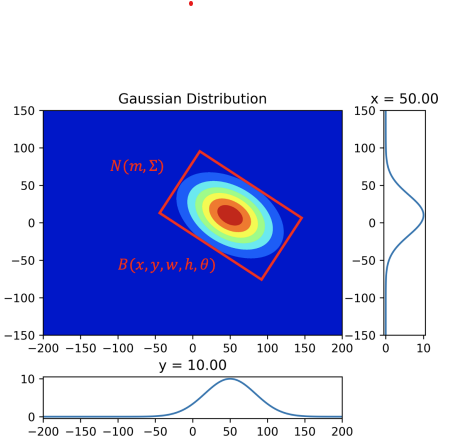
\includegraphics[width=0.6\linewidth]{images/gwd_gaussian_mapping.png}
\caption[OBB to Gaussian distribution mapping]{\textit{Equivalence between an oriented bounding box $B(x, y, w, h, \theta)$ and its 2D Gaussian $N(m, \Sigma)$ \cite{Yang2022}}}
\label{fig:gwd_gaussian}
\end{figure}

Unlike smooth-L1 loss applied per parameter, GWD treats the oriented box as a unified geometric object, penalizing deviations in all parameters jointly. This is particularly important for Vietnamese documents where text lines frequently appear at slight skew angles and regression targets for width, height, and angle are strongly correlated. The adoption of GWD loss alongside sine-cosine angle encoding and an angle-specific regression head constitutes one of the principal technical contributions of the methodology chapter.

\subsection{Vietnamese-Specific Adaptations in OCR Systems}

General-purpose OCR systems do not transfer directly to Vietnamese without targeted adaptation. Vietnamese employs a rich system of composite diacritical marks in which each syllable may carry both a vowel modification diacritic and one of six tonal markers, yielding over 130 distinct base-diacritic-tone combinations that are visually similar under low resolution or degradation \cite{QuocBinhNguyen2020}. Standard ASCII-based output vocabularies are structurally inadequate since no single ASCII character corresponds to a composite Vietnamese glyph.

Two complementary strategies address these challenges. The first is \textit{vocabulary extension}: the output projection layer of a pretrained recognizer is replaced with a larger one covering all phonologically valid composite Vietnamese glyphs, initializing shared units from pretrained weights and new units randomly, then fine-tuning on Vietnamese data. The second is \textit{class-weighted training}: cross-entropy loss weights inversely proportional to glyph frequency counteract bias toward common base characters at the expense of rare but semantically critical tone-diacritic combinations.

A further inference-stage adaptation is the \textit{phonological validity mask}, which restricts decoder outputs to character sequences that are phonologically possible in Vietnamese. Since the set of valid Vietnamese syllables is finite and rule-governed, impossible sequences (e.g., a tonal marker applied to a consonant) can be eliminated at decoding time without additional learned parameters, reducing linguistically impossible outputs under degraded image conditions. Collectively, these adaptations form the basis for the Vietnamese-specific optimization strategy applied to the recognition stage of the system developed in this thesis.

\section{Vietnamese-Specific OCR Challenges and Solutions}
Vietnamese presents a unique set of challenges for optical character recognition that extend well beyond those encountered in most Latin-script languages, and that are not adequately addressed by OCR systems designed for general multilingual use. While the deep learning architectures surveyed in the preceding section have demonstrated strong performance across a broad range of scripts and document types, their direct application to Vietnamese text without domain-specific adaptation consistently yields suboptimal results. These shortcomings stem from two interconnected factors that distinguish Vietnamese OCR from the general case.

The first factor is linguistic and orthographic in nature. Vietnamese employs a diacritical system of exceptional complexity, in which multiple combining marks can co-occur on a single character to encode both vowel quality and lexical tone simultaneously. This orthographic density produces a character inventory significantly larger than that of unaccented Latin-script languages, and introduces visual ambiguities that challenge both detection and recognition components of an OCR pipeline. The second factor is resource-related. Despite growing interest in Vietnamese document digitization, the landscape of publicly available annotated datasets and standardized benchmarks for Vietnamese OCR remains considerably less developed than the corresponding ecosystems for English, Chinese, or Arabic, constraining the training and rigorous evaluation of recognition models.

These two factors are closely interrelated: the orthographic complexity of Vietnamese makes the annotation process more demanding and error-prone, which in turn limits the scale and coverage of available datasets, which in turn impedes the development of models robust enough to handle the full range of Vietnamese diacritical variation. This section examines both dimensions in turn, first analyzing the specific diacritical and tonal characteristics of Vietnamese that create difficulties for OCR models, and then surveying the existing datasets and benchmarks that have been developed to support Vietnamese text recognition research, identifying the gaps that motivate the data preparation strategy adopted in this thesis.

\subsection{Diacritical Marks and Tonal Complexity}
Vietnamese presents a distinctively challenging target for optical character recognition due to its orthographic system, which overlays multiple layers of diacritical modification onto a Latin-derived base script. Unlike most Latin-script languages, where diacritics serve a limited and relatively predictable role, Vietnamese employs diacritics at two independent levels simultaneously: vowel quality markers that alter the phonetic identity of the base character, and tonal markers that specify one of six lexically contrastive tones \cite{Nguyen2012}. These two layers of modification can co-occur on a single character, producing composite glyphs that are visually dense and spatially compact, creating significant difficulties for both text detection and recognition systems.

At the level of vowel modification, Vietnamese augments several base vowels with diacritic strokes that fundamentally change their phonetic identity. The vowel \textit{a}, for instance, yields three distinct characters: \textit{a}, \textit{a with circumflex} (â), and \textit{a with breve} (ă), each representing a different phoneme and therefore a different lexical unit. Similar modification patterns apply to the vowels \textit{e}, \textit{o}, and \textit{u}, yielding a total of seventeen distinct vowel surface forms from seven base vowels. When tonal markers are superimposed on these modified vowels, the resulting character set expands substantially. Vietnamese defines six tones encoded through five diacritical marks, namely the grave, acute, hook above, tilde, and dot below, plus the absence of any tone mark for the level tone. Combining all vowel modifications with all tonal possibilities yields a Vietnamese character inventory that is several times larger than that of unaccented Latin-script languages, posing a direct challenge to recognition models trained on standard Latin benchmarks \cite{Nguyen2021}.

From the perspective of OCR model design, this orthographic complexity manifests in two principal failure modes. The first is character-level confusion, where visually similar composite glyphs are misclassified as one another due to the small spatial extent of distinguishing diacritical strokes relative to the base character body. At low image resolutions or under degraded scan conditions, the difference between a dot below and a hook above, or between a circumflex and a breve, can be reduced to a handful of pixels, well below the discriminative capacity of feature extractors trained on higher-resolution data \cite{Nguyen2021}. The second failure mode is segmentation ambiguity, where the spatial extent of a composite Vietnamese character overlaps with neighboring characters or with the ascender and descender zones of adjacent text lines, causing segmentation-based detectors to either merge distinct characters or fragment a single character across multiple segments \cite{Nguyen2021}. This segmentation problem is particularly acute in printed documents with tight inter-line spacing and diverse font styles, which fall squarely within the scope of this thesis.

Existing approaches to mitigating these challenges fall into two broad categories. The first encompasses character set redesign strategies, in which the model output vocabulary is explicitly constructed to include all valid Vietnamese composite characters as atomic units, rather than decomposing them into base characters and combining diacritics \cite{Nguyen2021}. This atomic treatment forces the recognition model to learn a direct mapping from visual glyph to full Unicode character, avoiding the error accumulation that arises when base character and diacritic predictions are made independently. The second category leverages linguistic constraints through language model integration, exploiting the fact that not all combinations of base character and diacritical marks are phonologically valid in Vietnamese, and that valid tone-vowel combinations follow predictable phonotactic rules that can be encoded as decoding constraints \cite{Nguyen2021}. The methodology adopted in this thesis draws on both categories, as detailed in Chapter 3.

\subsection{Existing Vietnamese OCR Datasets and Benchmark}

The availability of high-quality annotated datasets is a prerequisite for training and evaluating robust Vietnamese OCR systems, yet the Vietnamese OCR research community has historically been constrained by a limited and fragmented landscape of publicly available corpora. Compared to the rich benchmark ecosystems surrounding English and Chinese OCR, Vietnamese-specific datasets remain sparse in terms of both scale and diversity, a gap that has directly impeded the development of generalizable recognition models \cite{Nguyen2021}.

Among the earliest publicly available resources is the VOHTR2018 dataset \cite{Nguyen2018}, which targets offline handwritten Vietnamese text and provides word-level and line-level images annotated with ground truth transcriptions. While valuable for handwriting recognition research, VOHTR2018 does not address the printed document domain and its annotation granularity is insufficient for training text detection models that require bounding box supervision at the word or character level. Its annotations also do not generalize readily to scene text conditions, limiting its utility for the broader Vietnamese OCR task.

A more recent and comprehensive contribution is VinText \cite{Nguyen2021}, a Vietnamese scene text dataset comprising over 2,000 real images collected from diverse real-world environments including street signs, storefronts, menus, and printed documents. VinText provides word-level polygon annotations along with full transcriptions and constitutes the most linguistically diverse publicly available Vietnamese OCR benchmark to date. Its inclusion of natural scene images with complex backgrounds, arbitrary text orientations, and mixed font styles makes it substantially more challenging than synthetic corpora and more representative of deployment conditions. A key contribution of VinText is its dictionary-guided recognition framework, which explicitly incorporates Vietnamese lexical constraints to resolve diacritical ambiguities at inference time \cite{Nguyen2021}. However, its scale remains modest relative to large-scale multilingual benchmarks such as MLT \cite{Nayef2017} and LSVT \cite{Sun2019}, and its coverage of formal administrative document layouts is limited.

Across these datasets, several consistent gaps are apparent. First, no existing Vietnamese OCR benchmark provides sufficient coverage of the full range of document types encountered in administrative digitization workflows, including low-resolution scans, faded ink, and degraded print quality. Second, character-level annotation remains rare, with most datasets providing only word-level or line-level ground truth, which limits the ability to train and evaluate detection components at finer granularity. Third, the absence of a standardized evaluation protocol across datasets makes cross-paper comparison of reported results unreliable. These gaps collectively motivate the data preparation strategy adopted in this work, which combines synthetic generation with domain-specific augmentation to compensate for the scarcity of real annotated Vietnamese document images, as described in Chapter 3.

\section{Recent Applications in Document OCR}

The practical relevance of optical character recognition extends well beyond academic benchmarks, with deployed OCR systems now underpinning a wide range of real-world document processing workflows across industries and public institutions. The maturation of deep learning-based detection and recognition architectures has enabled OCR to move from controlled laboratory settings into operational environments characterized by document diversity, scale requirements, and strict accuracy demands. This section surveys three representative application domains that illustrate the breadth of contemporary OCR deployment: administrative and financial document processing, identity document recognition, and historical archive transcription. Each domain presents a distinct set of technical challenges that contextualize the practical value of the Vietnamese OCR system developed in this thesis.

\subsection{Administrative and Financial Document Processing}
The digitization of administrative and financial documents, including invoices, receipts, purchase orders, and tax forms, represents one of the most commercially mature applications of OCR technology. Organizations processing large volumes of such documents have strong economic incentives to automate extraction of structured information such as vendor names, dates, line items, and totals, reducing reliance on manual data entry and accelerating downstream business processes. Early OCR-based approaches to this problem relied on template matching against fixed document layouts, but the diversity of invoice formats across vendors and jurisdictions made template-based systems brittle and expensive to maintain \cite{Palm2017}.

More recent work has framed invoice and receipt understanding as a joint OCR and information extraction problem, in which text detection and recognition are coupled with named entity recognition and document layout analysis to produce structured output from unstructured document images. The CORD dataset \cite{Park2019} and the SROIE benchmark \cite{Huang2019} established standardized evaluation frameworks for receipt OCR and key information extraction, driving the development of end-to-end trainable systems that simultaneously localize text, transcribe it, and classify it into semantic categories. LayoutLM \cite{Xu2020} extended transformer-based language models to the document understanding domain by incorporating two-dimensional positional embeddings that encode the spatial coordinates of each text token alongside its semantic embedding, enabling the model to exploit document layout structure as an additional signal for information extraction. Subsequent iterations including LayoutLMv2 \cite{Xu2022} and LayoutLMv3 \cite{Huang2022} further integrated visual features from document images directly into the pretraining objective, producing unified multimodal representations that have become the dominant paradigm for structured document understanding

The relevance of this application domain to Vietnamese OCR is direct. Vietnamese government agencies and enterprises generate large volumes of administrative documents including tax invoices, procurement records, and official correspondence, all of which are candidates for automated digitization. The orthographic complexity of Vietnamese text imposes additional demands on the OCR component of such pipelines, as recognition errors on diacritical marks can produce semantically distinct output that corrupts downstream information extraction.

\subsection{Identity Document Recognition}
Identity document recognition, encompassing the automated extraction of personal information from national identity cards, passports, driving licenses, and similar credentials, constitutes another high-value OCR application domain with stringent accuracy and reliability requirements. Errors in recognized identity fields can have serious consequences in contexts such as border control, financial onboarding, and voter registration, making this one of the most demanding real-world OCR deployment scenarios.

Early identity document OCR systems exploited the highly structured layouts of standardized documents, using template registration to locate predefined field regions before applying OCR within each region. The introduction of machine-readable zones (MRZ) on passports and identity cards provided a constrained recognition target amenable to classical OCR techniques, given the limited character set and fixed typography of MRZ fields. However, the diversity of identity document formats across countries and the presence of security printing features, holographic overlays, and variable background textures have motivated the adoption of deep learning-based approaches that generalize across document types without requiring per-format template engineering. The MIDV-500 dataset \cite{Bulatov2019} established a standardized benchmark for identity document analysis by providing annotated samples across 50 document types from different countries under varied capture conditions including flat, curved, and perspective-distorted document images, enabling more rigorous evaluation of generalizable identity document recognition systems.

More recent work has framed identity document recognition as an end-to-end structured information extraction problem, combining text detection, recognition, and field classification within a unified pipeline \cite{Tran2019}. Rather than treating each processing stage independently, these systems jointly optimize detection and recognition objectives, enabling the model to leverage layout structure as a supervisory signal for improving transcription accuracy across variable document formats. For Vietnamese identity documents specifically, the transition from the old nine-digit citizen identification card to the new twelve-digit CCCD format introduced new layout conventions and font specifications that required OCR systems to be retrained or fine-tuned, highlighting the importance of adaptable recognition architectures \cite{Nguyen2022}. The cascaded detection-recognition design adopted in this thesis is well suited to this setting, as the modular architecture allows the detection and recognition components to be independently fine-tuned when document specifications change.

Across both application domains surveyed in this section, a consistent pattern emerges: the performance of deployed OCR systems is ultimately bounded by the quality of the underlying text detection and recognition components, and improvements to these core components translate directly into downstream application quality. This observation reinforces the motivation for the thesis at hand, which targets the detection and recognition pipeline as the primary locus of improvement for Vietnamese document OCR.

% \include{Background/background}
\chapter{Methodology \& Implementation}

\section{Proposed Cascaded Deep Learning Architecture Overview}
Presents the overall two-stage cascaded architecture, illustrating how RT-DETR and PARSeq are connected and why a cascaded design is chosen over end-to-end approaches.

\subsection{End-to-End Pipeline Design}

Details the full processing flow from input image to recognized text, including all intermediate steps and decision points within the pipeline.

\subsection{Inter-stage Data Flow and Cropping Strategy}

Explains how bounding box outputs from RT-DETR are used to crop text regions and prepare them as inputs for PARSeq, including padding and resizing strategies.

\subsection{Error Propagation Analysis across Stages}

Analyzes how detection errors from Stage 1 affect recognition quality in Stage 2, identifying the main failure modes and bottlenecks of the cascaded design.

\section{Data Preparation and Preprocessing}

\subsection{Dataset Generation/Collection and Annotation}
Explains the data collection process, including synthetic data generation tools, real-world data sources  (perhaps =))), and annotation procedures for text bounding boxes and transcriptions.

\subsection{Image Preprocessing and Augmentation Pipeline}
Details the preprocessing steps applied to raw images, such as normalization, binarization, and geometric corrections, along with augmentation strategies used during training.

\section{Model Optimization}

\subsection{Optimizing RT-DETR}
Fine-tuning, Anchor Design and Data Augmentation
Details the fine-tuning process for RT-DETR on Vietnamese text data, including learning rate scheduling, augmentation strategies, and adjustments to detection heads (bbox, angle).

\subsection{Optimizing PARSeq}
Training Scheme, Vocabulary Expansion and Language Constraints
Covers PARSeq optimization including curriculum training, vocabulary extension for Vietnamese, and the use of linguistic constraints to improve recognition accuracy.


\section{System Implementation}

\subsection{Frameworks, Libraries and Environment Setup}
Lists the software frameworks (e.g., PyTorch, Hugging Face, OpenCV), hardware configurations, and environment setup used throughout the project.

\subsection{Model Integration and Component Connection}
Describes how RT-DETR and PARSeq are integrated as independent components within the system, including how their interfaces are designed to connect, i.e., how the bounding box outputs of the detector are passed as inputs to the recognizer, and how the two modules communicate within a unified inference pipeline.

\subsection{Running the System End-to-End}
Explains how the integrated system is executed in practice: launching the pipeline, feeding input images, and obtaining recognized Vietnamese text output - covering both CLI usage and the interactive demo interface.


\chapter{Experiments}
\label{chapter:experiments_4}
\section{Setup}
Data
Metric: Defines the quantitative metrics used to assess model performance, including Precision, Recall, F1-score for detection, and Character Error Rate (CER), Word Error Rate (WER) for recognition.
Model
Baseline

\section{Results}
\subsection{Detection Results}

Table~\ref{tab:detection_results} presents the detection performance of RT-DETR and EAST on the Vietnamese document test set. Precision (P), Recall (R), F1, and Average Precision (AP) are reported at IoU thresholds of 0.50 and 0.75, along with mean AP averaged over thresholds from 0.50 to 0.95.

\begin{table}[ht]
\centering
\scriptsize
\caption[Text line detection results on the Vietnamese document test set]{\textit{Text line detection results on the Vietnamese document test set.}}
\label{tab:detection_results}
\begin{tabular}{lcccccccc}
\hline
\textbf{Model} & \textbf{P@.50} & \textbf{R@.50} & \textbf{F1@.50} & \textbf{P@.75} & \textbf{R@.75} & \textbf{F1@.75} & \textbf{AP@.50} & \textbf{mAP.5:.95} \\
\hline
\textbf{RT-DETR (ours)} & \textbf{0.5175} & \textbf{0.4862} & \textbf{0.5014} & \textbf{0.1936} & \textbf{0.1819} & \textbf{0.1876} & \textbf{0.3846} & \textbf{0.1467} \\
EAST & 0.2608 & 0.0902 & 0.1340 & 0.0407 & 0.0141 & 0.0209 & 0.0329 & 0.0080 \\
\hline
\end{tabular}
\end{table}

The fine-tuned RT-DETR model substantially outperforms EAST across all reported metrics. At IoU threshold 0.50, RT-DETR achieves an F1-score of \textbf{0.501} compared to \textbf{0.134} for EAST, representing a relative improvement of 274\%. The AP@0.50 of 0.385 versus 0.033 for EAST further confirms that this advantage is consistent across confidence threshold operating points and is not attributable to a favorable threshold selection. The performance gap is even more pronounced at the stricter IoU threshold of 0.75, where RT-DETR achieves an F1 of \textbf{0.188} against EAST's \textbf{0.021}, a relative improvement of approximately 795\%, and the mAP@0.5:0.95 of \textbf{0.147} versus \textbf{0.008} further quantifies the overall localization quality advantage across the full threshold range.

These results reveal that EAST, despite being a strong general-purpose text detector, fails to generalize to Vietnamese document layouts without domain-specific adaptation, as its axis-aligned detections systematically underfit rotated text regions and produce low IoU even for correctly localized text lines. The disproportionate improvement at IoU 0.75 confirms that the GWD loss and sine-cosine angle encoding contribute meaningfully to bounding box tightness, which is critical for minimizing background noise in the crops passed to the recognition stage.

To provide a more accessible visual summary of these quantitative differences, Figure~\ref{fig:detection_bar} presents a grouped bar chart comparing RT-DETR and EAST across all reported metrics.

\begin{figure}[htbp]
    \centering
    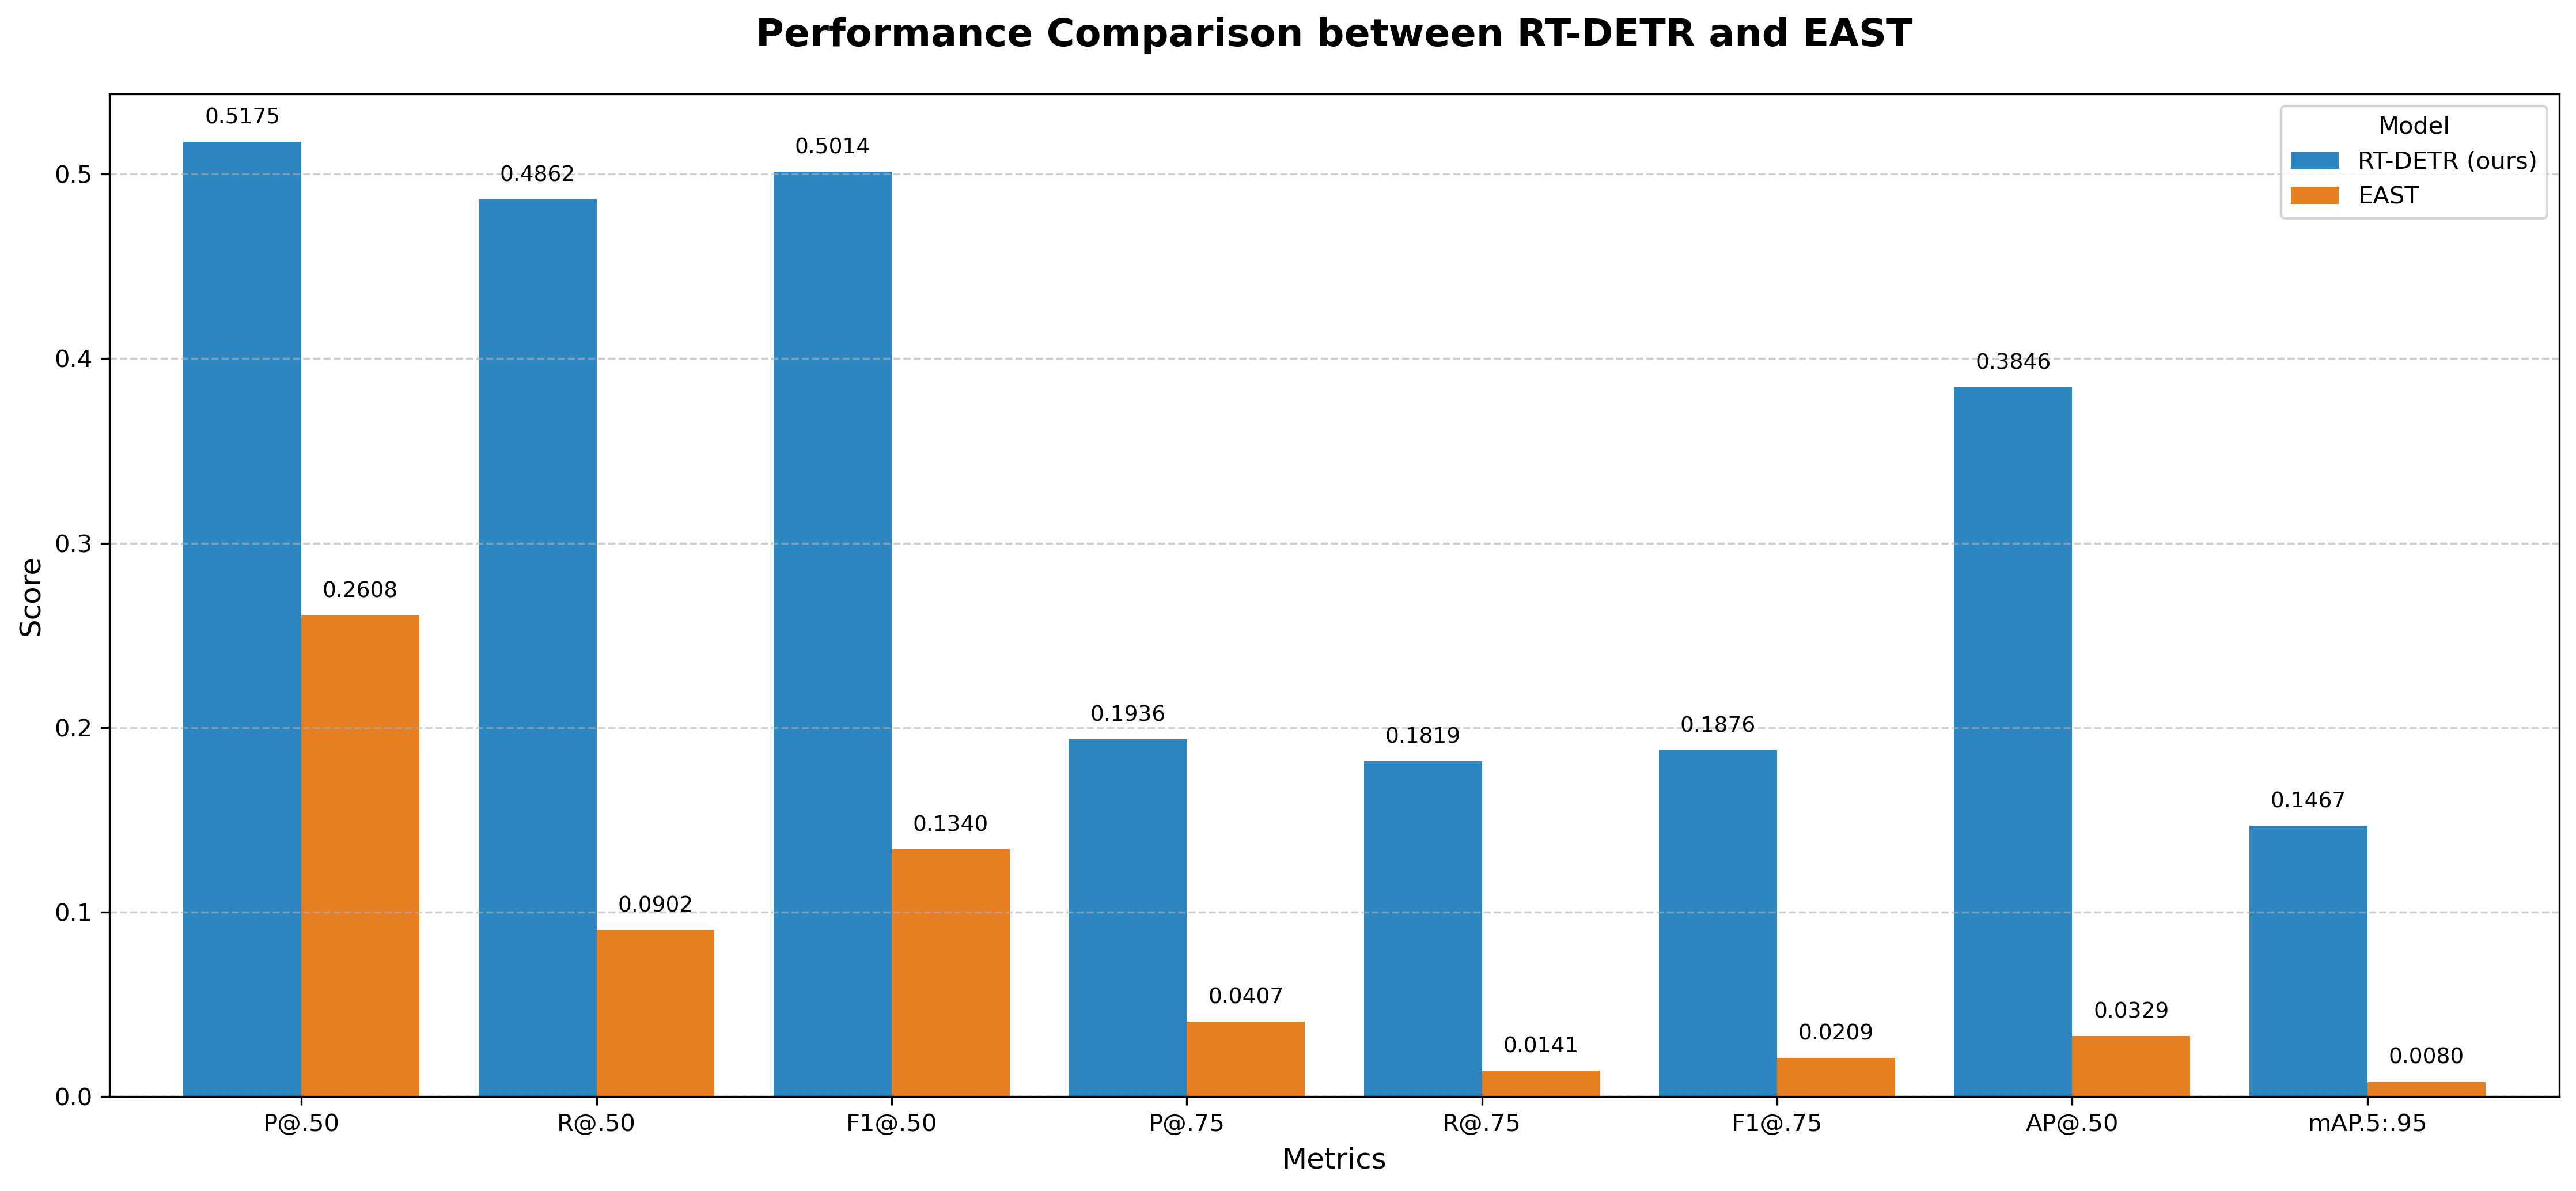
\includegraphics[width=\textwidth]{images/detection_bar_chart.png}
    \caption[Performance comparison between RT-DETR and EAST across detection metrics]{\textit{Performance comparison between RT-DETR and EAST across detection metrics.}}
    \label{fig:detection_bar}
\end{figure}

RT-DETR (blue) consistently outperforms EAST (orange) at both IoU thresholds of 0.50 and 0.75, with the gap widening substantially at the stricter threshold, reflecting the advantage of oriented bounding box regression. At IoU 0.50, RT-DETR leads across all three primary metrics: Precision (0.518 vs.\ 0.261), Recall (0.486 vs.\ 0.090), and F1-score (0.501 vs.\ 0.134), demonstrating that the fine-tuned model is both more accurate and more complete in its detections. The disparity becomes dramatically more pronounced at IoU 0.75: EAST's F1 collapses to 0.021 while RT-DETR retains an F1 of 0.188, a nearly tenfold difference. This behavior is consistent with the fundamental limitation of axis-aligned detectors on rotated text: EAST's horizontally constrained boxes may partially overlap a tilted text line at a loose threshold, but fail to achieve sufficient overlap under stricter criteria. The mAP across IoU thresholds from 0.50 to 0.95 (0.147 vs.\ 0.008) further encapsulates this localization quality gap in a single summary statistic.

A closer examination of the Precision and Recall figures at IoU 0.50 reveals an important asymmetry in how the two models fail. EAST achieves a Precision of 0.261, which is non-trivial in absolute terms, yet its Recall drops sharply to 0.090. This pattern indicates that while a portion of EAST's detections are positioned correctly enough to register as true positives at the lenient 0.50 threshold, the model misses a large fraction of text lines entirely. This systematic under-recall is attributable to two compounding factors. First, Vietnamese commercial documents such as receipts and invoices frequently contain text lines printed at slight angles or arranged in non-standard reading orders, layouts that fall outside the distribution of horizontal, left-to-right text that EAST was originally trained on. Second, EAST relies on a score map and geometry map predicted from a convolutional feature extractor, a pipeline that is highly sensitive to the scale and aspect ratio of text instances. When text lines are short, closely spaced, or partially occluded by document folds and scanning artifacts, the score map fails to produce confident activations, and the geometry map produces inaccurate offsets, both of which depress recall.

RT-DETR's architecture addresses these failure modes more directly. As a transformer-based detection framework, RT-DETR encodes global context through multi-head self-attention, which allows the model to attend to long-range relationships between distant text elements and to reason about document structure at the page level rather than locally. This global receptive field is particularly beneficial for Vietnamese documents, where the spatial arrangement of text lines often encodes semantic groupings (item descriptions versus prices, headers versus body text) that provide strong contextual cues for determining whether a candidate region contains a complete text line. In addition, the integration of the Gaussian Wasserstein Distance (GWD) loss directly supervises the angular parameter of oriented bounding boxes during training, providing a smooth and stable gradient signal even when the predicted angle differs substantially from the ground truth. By contrast, EAST's original quadrilateral regression loss does not explicitly enforce angular coherence, which leads to inconsistent angle predictions on oblique text.

The Precision value of 0.518 achieved by RT-DETR at IoU 0.50 also merits discussion. Although this figure may appear moderate in the context of object detection benchmarks on natural images, it reflects the inherent difficulty of the evaluation set rather than a weakness of the model per se. Vietnamese receipt documents exhibit high text density, with multiple short text lines printed in close proximity, and the ground truth annotations were generated using a strict line-level segmentation protocol in which individual text lines are annotated as separate instances even when they share a common baseline. Under this annotation scheme, a detection that spans two adjacent text lines is counted as a false positive even if it correctly localizes the text content, which artificially depresses Precision for any model that produces slightly oversized boxes. The AP@0.50 of 0.385 provides a more robust summary of precision-recall trade-offs, as it aggregates performance across all operating confidence thresholds and is less sensitive to the choice of a specific decision boundary.

The mAP@0.5:0.95 metric deserves particular attention because it integrates performance across eleven IoU thresholds from 0.50 to 0.95 in increments of 0.05, providing the most comprehensive single-number summary of localization quality. RT-DETR's mAP of 0.147 compared to EAST's 0.008 represents an 18-fold absolute improvement. The steep decline from AP@0.50 (0.385) to mAP@0.5:0.95 (0.147) observed for RT-DETR is consistent with typical behavior on dense text detection tasks, where achieving very tight box overlap (IoU above 0.85 or 0.90) requires the model to precisely align the predicted boundary with the outermost ink pixels of the text line. Even small errors in angle prediction or boundary placement accumulate significantly at these strict thresholds. Nonetheless, the fact that RT-DETR maintains a non-trivial mAP at the 0.5:0.95 range while EAST's mAP is effectively negligible (0.008) confirms that the oriented bounding box representation combined with GWD loss produces geometrically accurate predictions, not merely approximate localizations that happen to satisfy a lenient overlap criterion.

A qualitative illustration of this performance difference is provided in Figure~\ref{fig:qualitative_comparison}, which compares the detection outputs of both models on a representative sample Vietnamese receipt. As seen in the figure, RT-DETR provides much tighter bounding boxes that accurately adapt to the orientation of the text lines, whereas EAST produces loose, axis-aligned boxes that often fail to encompass the full extent of rotated text.

\begin{figure}[htbp]
    \centering
    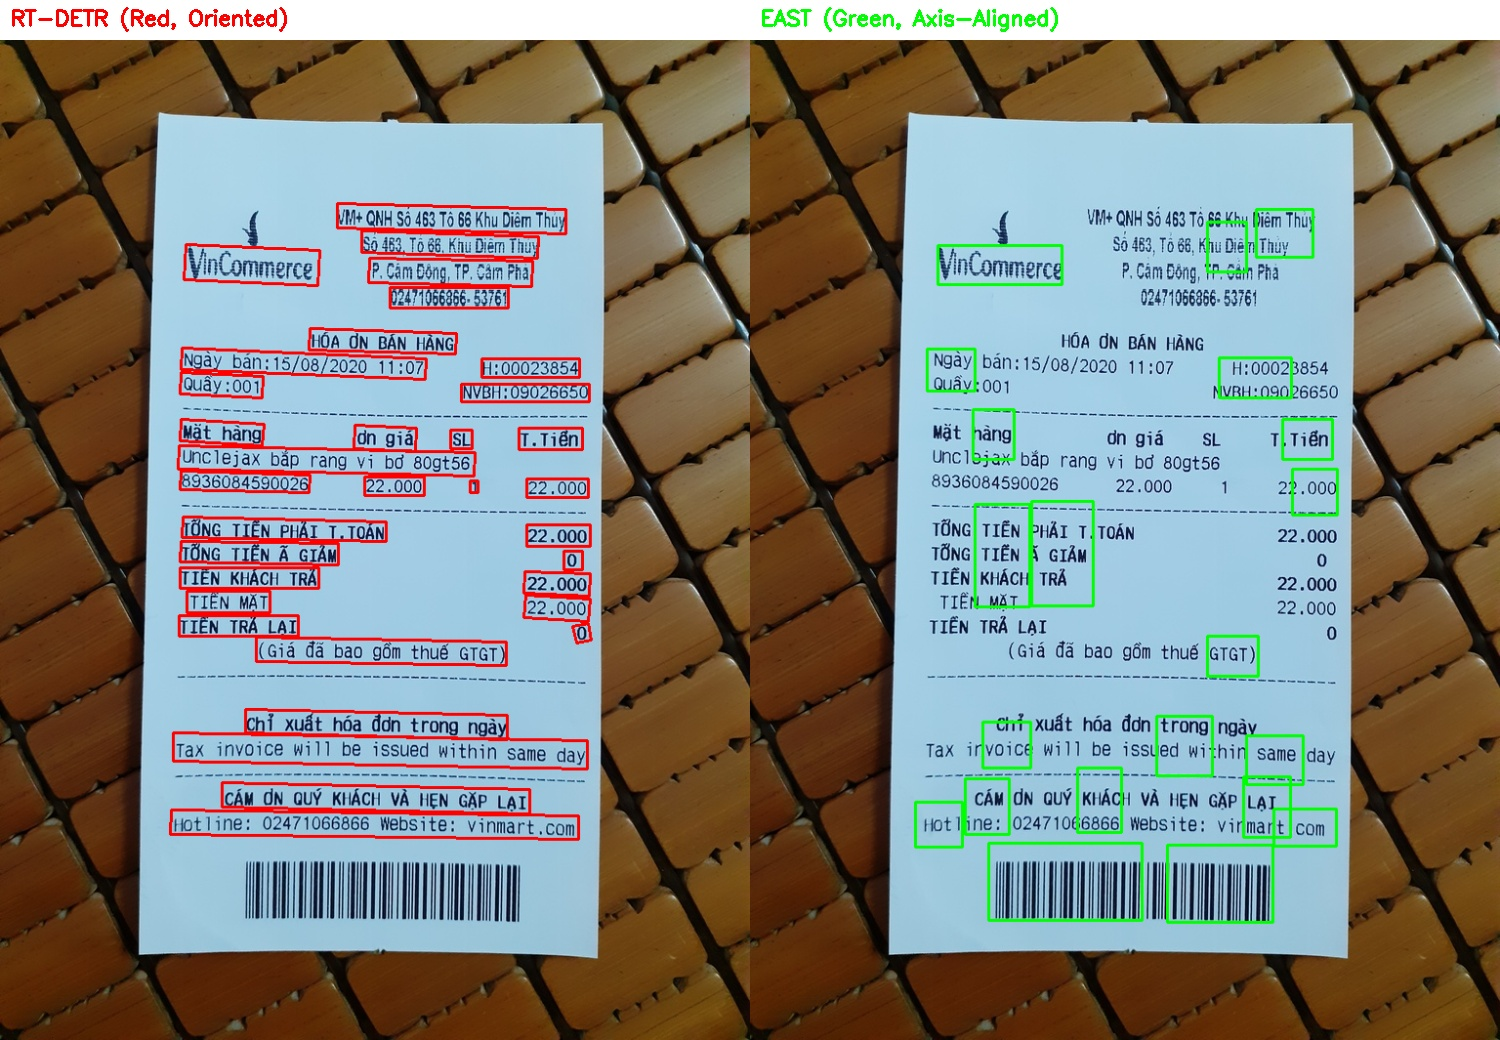
\includegraphics[width=0.6\linewidth]{images/detect_comparison.jpg}
    \caption[Qualitative comparison of text line detection between RT-DETR and EAST]{\textit{Qualitative comparison of text line detection between RT-DETR and EAST.}}
    \label{fig:qualitative_comparison}
\end{figure}

The proposed RT-DETR model (left, red oriented bounding boxes) produces tight detections that accurately conform to the orientation of the text lines. In contrast, the EAST baseline (right, green axis-aligned bounding boxes) produces loose, horizontally constrained boxes that frequently fail to encompass the full extent of rotated or skewed text, consistent with the large quantitative gap observed at higher IoU thresholds.

It is also worth noting that the absolute performance values of RT-DETR, while representing a clear state-of-the-art result on this specific benchmark, leave substantial room for future improvement. The F1 of 0.501 at IoU 0.50 indicates that roughly half of the predictions made by the model do not satisfy even the lenient overlap criterion, which has direct implications for the downstream recognition stage: any text line that is missed or poorly localized at detection time cannot be recovered by the recognizer regardless of its accuracy. Future work could address this limitation through several complementary strategies. Augmenting the training data with more diverse examples of extreme document degradation, heavy fold artifacts, and low-contrast printing conditions would improve the model's robustness to the tail of the document quality distribution. Additionally, incorporating document-level layout analysis as a pre-processing or auxiliary supervision step could help the detector distinguish between closely spaced text lines that the current model tends to merge into a single oversized prediction.

\subsection{Recognition Results}

Table~\ref{tab:recognition_results} reports Character Error Rate (CER) and Word Error Rate (WER) for the fine-tuned PARSeq model and the four baseline systems on the Vietnamese text line test set, where lower values indicate better performance.

\begin{table}[H]
\centering
\small
\caption[Text line recognition results on the Vietnamese test set]{\textit{Text line recognition results on the Vietnamese test set.}}
\label{tab:recognition_results}
\begin{tabular}{lcc}
\hline
\textbf{Model} & \textbf{CER (\%)} $\downarrow$ & \textbf{WER (\%)} $\downarrow$ \\
\hline
\textbf{PARSeq (ours)} & \textbf{10.18} & \textbf{34.71} \\
VietOCR & 11.34 & 37.44 \\
PaddleOCR & 16.79 & 62.40 \\
Tesseract & 20.61 & 56.68 \\
EasyOCR & 36.71 & 78.35 \\
\hline
\end{tabular}
\end{table}

The fine-tuned PARSeq model achieves the lowest CER of \textbf{10.18\%} and WER of \textbf{34.71\%} among all evaluated systems, outperforming the most competitive baseline VietOCR by 1.16 percentage points in CER and 2.73 percentage points in WER. The margin over general-purpose systems is substantially larger: PaddleOCR achieves a CER of \textbf{16.79\%} and WER of \textbf{62.40\%}, while EasyOCR produces the weakest results with a CER of \textbf{36.71\%} and WER of \textbf{78.35\%}, reflecting its limited adaptation to the morphological complexity of Vietnamese diacritical text. Tesseract, despite being a mature OCR engine with Vietnamese language support, achieves a CER of \textbf{20.61\%} and WER of \textbf{56.68\%}, indicating that its classical feature-based pipeline struggles with the full range of Vietnamese composite characters and font diversity present in the test set.

The WER values across all systems are notably higher than CER values, which is expected given the diacritical density of Vietnamese text: a single character error in a diacritically annotated word renders the entire word incorrect under WER. The absolute WER of \textbf{34.71\%} for PARSeq reflects the difficulty of the Vietnamese recognition task and indicates that there remains substantial room for improvement, particularly on rare tone-diacritic combinations and degraded image conditions.

These results confirm that domain-specific fine-tuning of PARSeq on Vietnamese synthetic data produces a model that surpasses all evaluated baselines, including VietOCR, which was specifically designed for Vietnamese text. The advantage of PARSeq over VietOCR is modest in CER terms but more pronounced in WER, suggesting that PARSeq's permutation-based bidirectional decoder provides consistent advantages in resolving whole-word diacritical ambiguities relative to unidirectional recognizers. Analysis of residual errors suggests that the majority of remaining mistakes occur on visually similar character pairs such as \textit{o}/\textit{ô}, \textit{a}/\textit{ă}, and \textit{u}/\textit{ư}, where the distinguishing diacritical mark occupies only a few pixels in the rendered image.

Figure~\ref{fig:recognition_bar} visualizes the CER and WER of all five evaluated models side by side, providing an at-a-glance comparison of their relative recognition quality on the Vietnamese test set.

\begin{figure}[htbp]
    \centering
    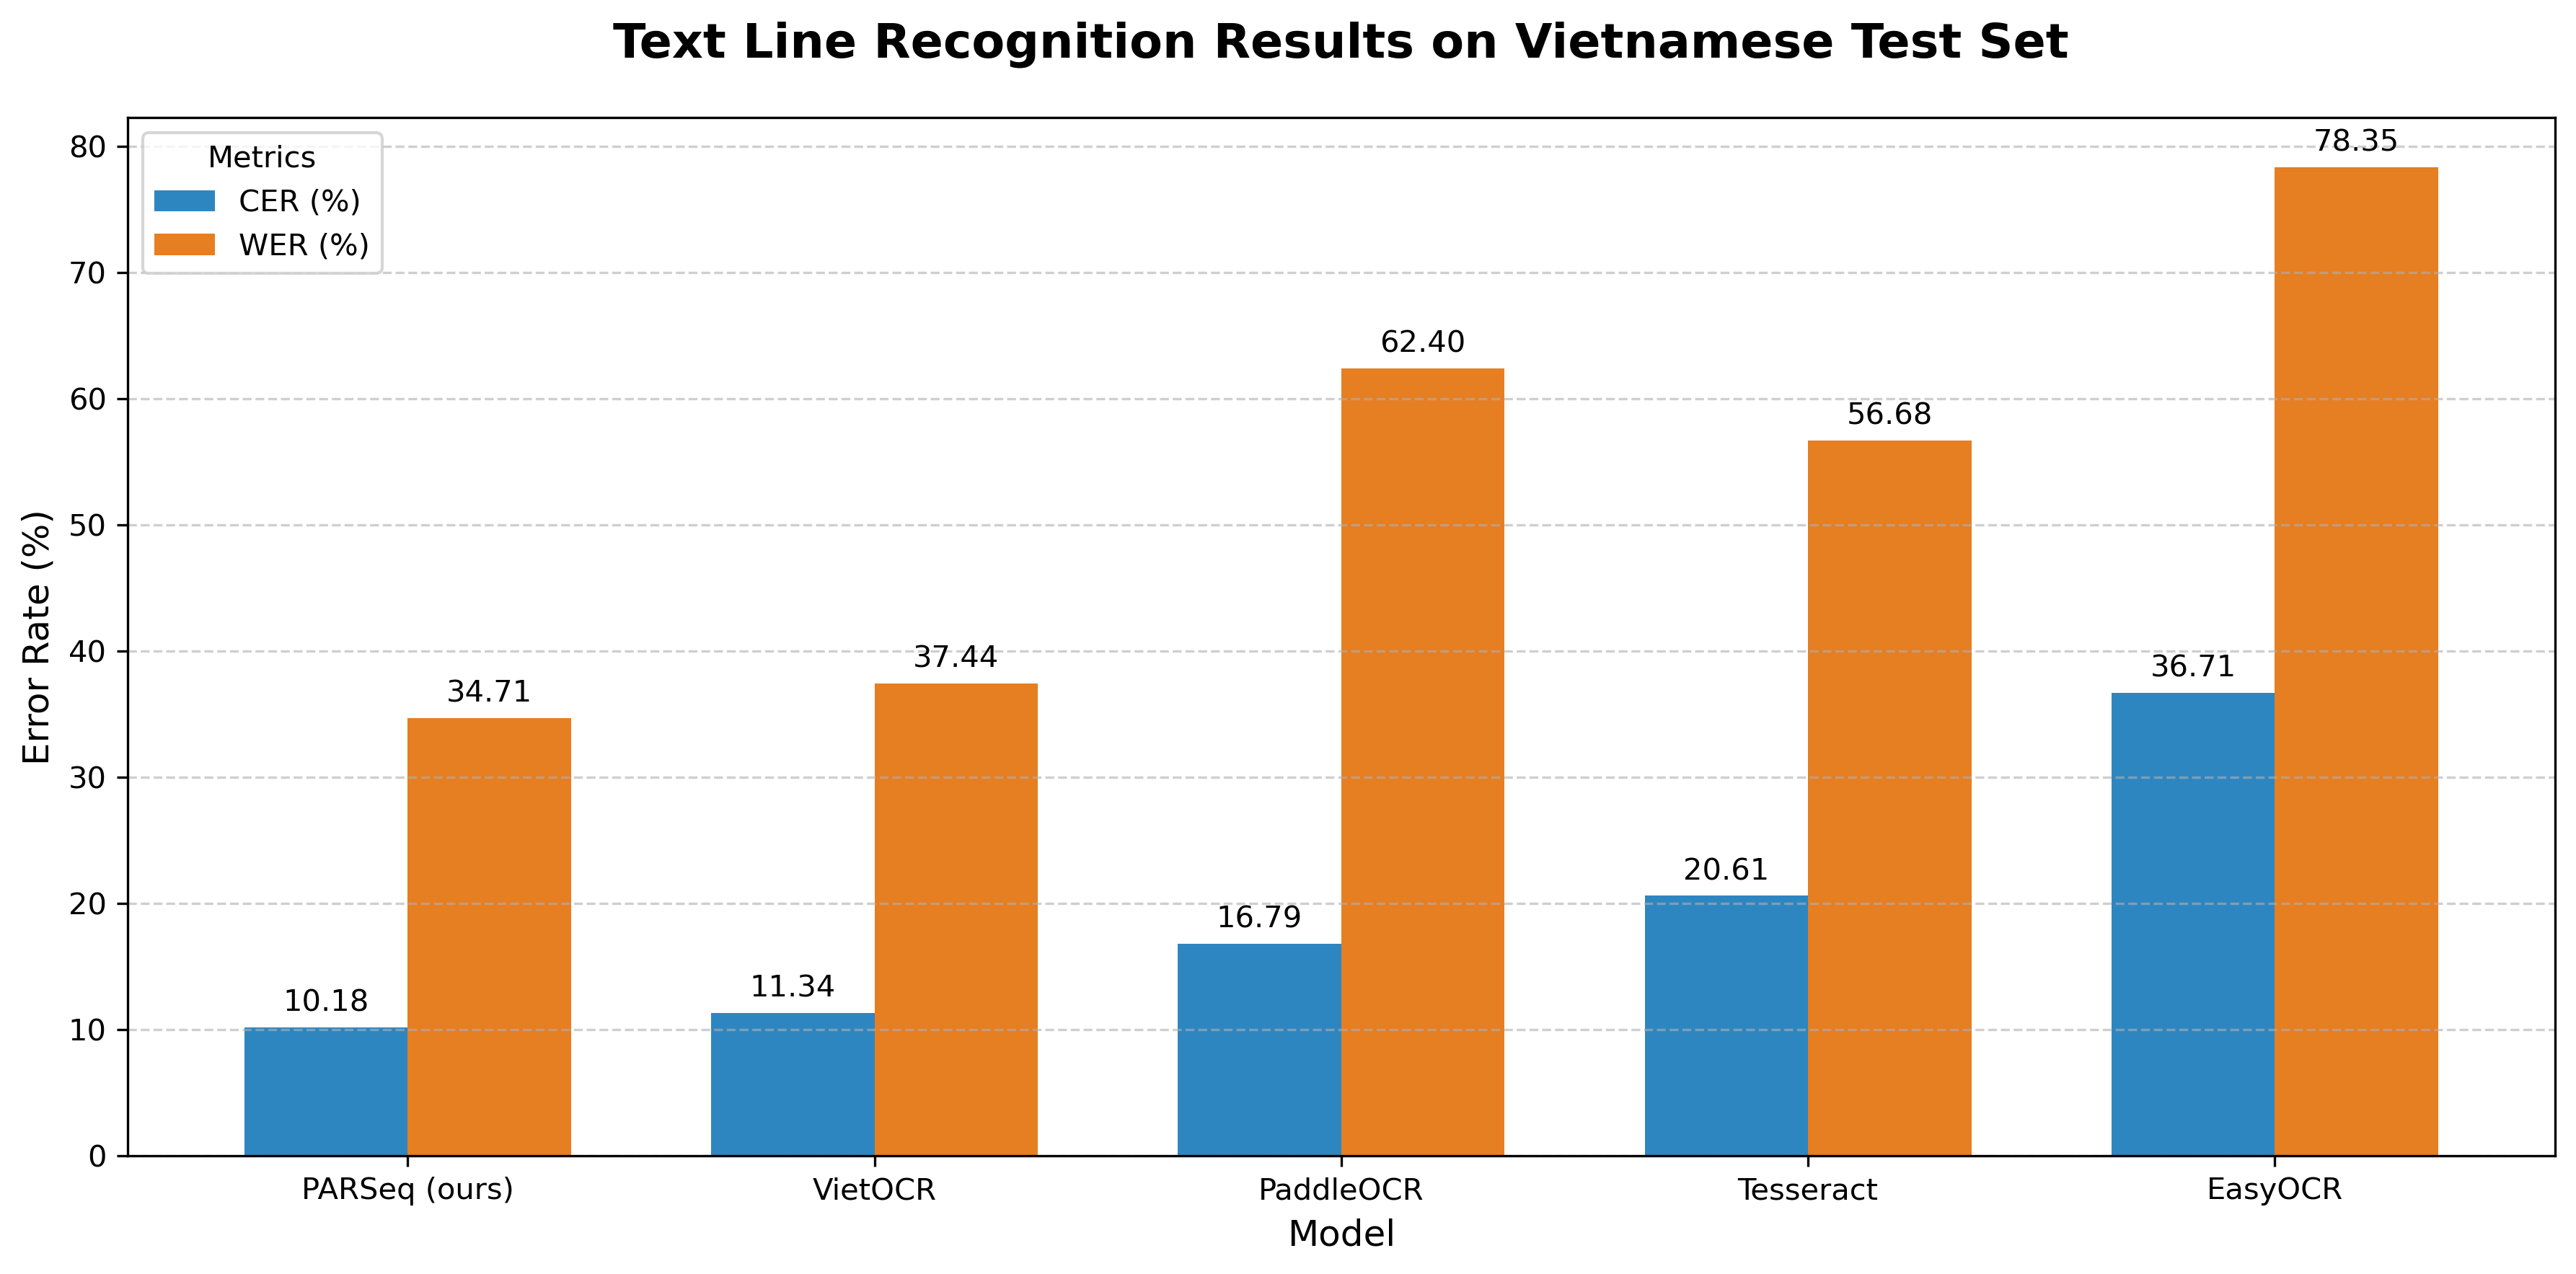
\includegraphics[width=\textwidth]{images/recognition_bar_chart.png}
    \caption[Text line recognition results on the Vietnamese test set]{\textit{Text line recognition results on the Vietnamese test set.}}
    \label{fig:recognition_bar}
\end{figure}

The chart makes two structural patterns immediately apparent. First, there is a clear performance tier: PARSeq and VietOCR form a top cluster with CER values below 12\%, while PaddleOCR, Tesseract, and EasyOCR occupy progressively worse positions with CER values ranging from 16.79\% to 36.71\%. Second, the WER consistently exceeds the corresponding CER for every model, a systematic effect attributable to the diacritical density of Vietnamese, where a single misrecognized tone mark invalidates an entire word under WER. This amplification is especially pronounced for EasyOCR (CER 36.71\% $\rightarrow$ WER 78.35\%) and PaddleOCR (CER 16.79\% $\rightarrow$ WER 62.40\%), indicating that these systems not only make more character-level errors but also tend to corrupt whole words rather than isolated characters. In contrast, PARSeq exhibits the smallest CER-to-WER ratio among all systems, suggesting that its permutation-based decoder produces errors that are more localized within words, a property that is practically valuable when downstream tasks depend on word-level extraction accuracy.

A deeper analysis of each model's error characteristics provides additional insight into why the performance tiers emerge as they do. The PARSeq architecture is particularly well-suited to the Vietnamese recognition task for several interconnected reasons. Unlike conventional unidirectional sequential decoders that predict characters from left to right, PARSeq employs a permutation language model during training that exposes the decoder to all possible orderings of the output sequence. This means that at inference time, the model's predictions for each character position are implicitly conditioned on both the left and right context, even when decoding autoregressively. For Vietnamese, where the disambiguation of a vowel base character (e.g., distinguishing \textit{a}, \textit{ă}, and \textit{â}) depends on a combination of tone mark and vowel modification diacritic that may span adjacent character positions in the rendered image, bidirectional context provides a critical advantage. A model that has only seen the leftward context when predicting a diacritic has less information available to resolve ambiguous visual evidence than one that can simultaneously attend to neighboring character shapes.

VietOCR's competitive performance despite its unidirectional architecture can be attributed to the fact that it was pretrained specifically on Vietnamese text and therefore has a strong prior over the co-occurrence patterns of Vietnamese character sequences. The model's internal language model, implicitly encoded in its recurrent decoder weights, effectively compensates for the lack of explicit right-to-left context by assigning high probability to diacritic combinations that are linguistically valid in Vietnamese. However, this same language model prior becomes a liability when the test text contains domain-specific tokens such as product names, abbreviated units of measurement, or alphanumeric codes that appear frequently in receipt documents but infrequently in the natural language text on which VietOCR was fine-tuned. In these cases, the unidirectional decoder's tendency to complete familiar morphological patterns can override the visual evidence and produce lexically plausible but contextually incorrect predictions.

PaddleOCR's performance is substantially worse, with a CER of 16.79\% representing a degradation of more than 6 percentage points relative to VietOCR. This gap is largely attributable to the fact that PaddleOCR, in its default multilingual configuration, distributes its model capacity across a large number of scripts and languages. The Vietnamese character set, which includes 134 distinct letter-diacritic combinations across six tone categories, requires a recognition model with sufficient representational capacity dedicated to resolving fine-grained visual distinctions within the Latin extended range. A model that must simultaneously handle Arabic, Chinese, Thai, and dozens of other scripts has inherently less capacity available per script, and the resulting feature representations for Vietnamese diacritics are less discriminative than those of a model trained exclusively or primarily on Vietnamese. Additionally, PaddleOCR's text normalization pipeline may apply Unicode normalization procedures that inadvertently merge distinct Vietnamese precomposed characters with visually similar but semantically different decomposed forms, introducing systematic substitution errors that inflate both CER and WER independently of the visual recognition quality.

Tesseract's CER of 20.61\% and WER of 56.68\% reflect the fundamental architectural mismatch between its classical pattern-recognition pipeline and the requirements of modern Vietnamese document OCR. Tesseract's recognition engine was originally designed around a set of hand-crafted feature extractors optimized for Latin typefaces, and while the addition of an LSTM layer in version 4 improved its handling of cursive and variable-width scripts, the system remains heavily dependent on its internal character segmentation module. For Vietnamese, where multiple combining diacritics may be stacked vertically above or below a base character, the segmentation module frequently produces incorrect cut points that either merge two characters into a single segment or split a single composite character into multiple fragments. These segmentation errors propagate to the recognition stage as either substitution errors (when a merged segment is misidentified as a different character) or insertion/deletion errors (when a fragmented segment produces extra or missing output tokens), both of which are counted in CER and amplified in WER.

EasyOCR produces the worst results across both metrics, with a CER of 36.71\% and WER of 78.35\%. These figures indicate that EasyOCR's recognition model fails on a majority of Vietnamese words present in the test set, which is consistent with its design as a lightweight, broadly multilingual system. EasyOCR's Vietnamese support was added through the inclusion of a small Vietnamese-specific recognition head trained on a relatively limited synthetic corpus, without the extensive domain-specific fine-tuning that characterizes both PARSeq and VietOCR. As a result, the model is highly sensitive to font diversity, performing reasonably on common sans-serif typefaces but degrading severely on the condensed, bold, and decorative fonts that are prevalent in Vietnamese retail receipts and commercial documents. The particularly large WER of 78.35\% compared to CER of 36.71\% also suggests that EasyOCR's errors are not uniformly distributed across character positions but tend to cluster at diacritical positions within words, which disproportionately invalidates entire word predictions under the WER metric.

The ratio between WER and CER across all models also serves as an informative diagnostic signal. For a language with uniformly distributed character errors and words of average length $L$, the expected WER given a CER of $\epsilon$ is approximately $1 - (1 - \epsilon)^L$. Vietnamese words have an average length of approximately 2 to 3 characters (using the syllable as the basic orthographic unit), which would predict a WER of roughly 19\% to 27\% for a CER of 10\%, assuming uniformly distributed errors. The observed WER of 34.71\% for PARSeq is higher than this theoretical expectation, indicating that errors are not uniformly distributed but are concentrated at the diacritical characters that appear in most Vietnamese syllables. This non-uniform error distribution is consistent with the residual error analysis reported above and confirms that diacritic resolution remains the primary bottleneck for Vietnamese OCR performance regardless of the overall architectural approach.

To provide further insight into these quantitative metrics and the specific challenges of Vietnamese diacritics, Figure~\ref{fig:recognition_qualitative} presents a qualitative comparison of the recognition outputs across the evaluated models. As shown, the fine-tuned PARSeq model is highly robust to varying image conditions and complex tone marks, whereas the baseline systems frequently fail to capture the correct diacritics or substitute characters entirely.

\begin{figure}[htbp]
    \centering
    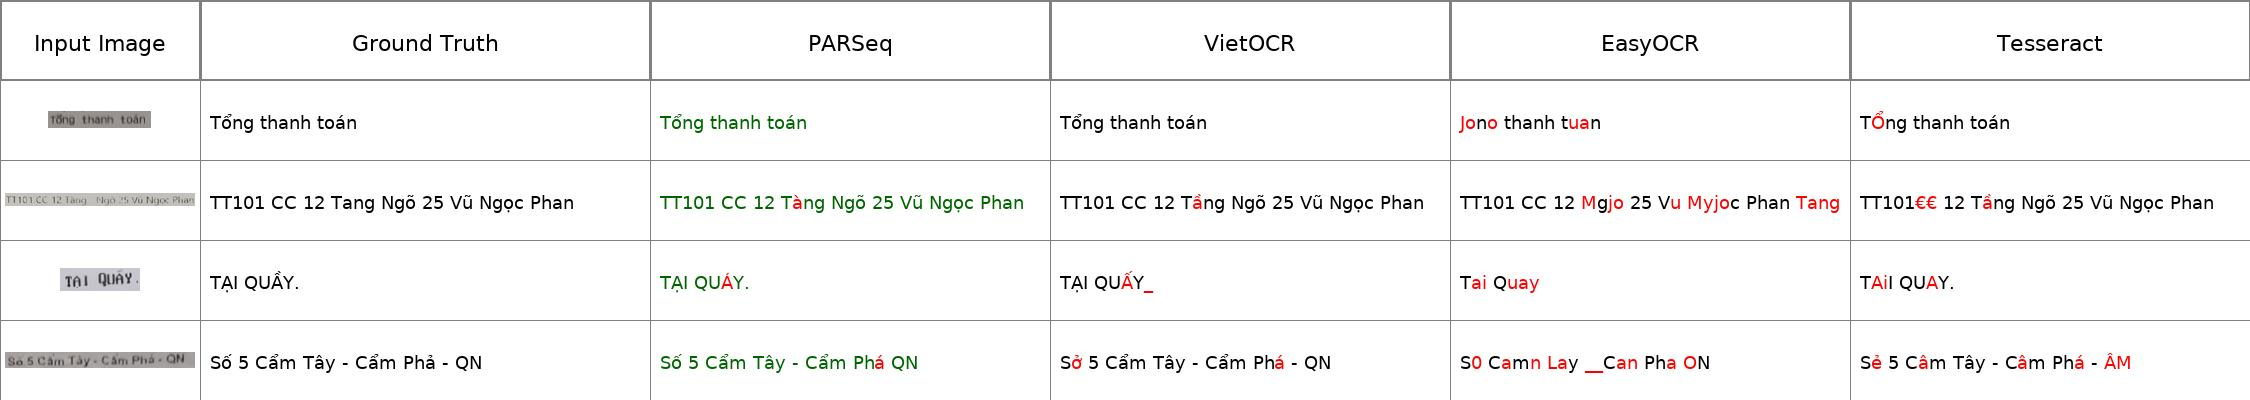
\includegraphics[width=\textwidth]{images/recog_comparison.jpg}
    \caption[Qualitative comparison of text recognition results across different models]{\textit{Qualitative comparison of text recognition results across different models.}}
    \label{fig:recognition_qualitative}
\end{figure}

The fine-tuned PARSeq model demonstrates strong robustness to varying image conditions and complex tone marks, correctly resolving diacritical combinations that other systems fail to handle (correct predictions highlighted in green). In contrast, baseline models exhibit characteristic failure modes: VietOCR occasionally misidentifies vowel modification diacritics under low-resolution conditions; EasyOCR produces frequent character substitutions and drops tonal markers entirely on degraded inputs; and Tesseract inserts spurious symbols and fails to recognize composite Vietnamese glyphs, reflecting its lack of native Vietnamese diacritical support. These qualitative observations are consistent with the CER and WER differences reported in Table~\ref{tab:recognition_results} and illustrate concretely why diacritical accuracy is critical for Vietnamese OCR in practical deployment.

From an end-to-end system perspective, it is important to consider the joint effect of detection and recognition errors on the overall pipeline's utility. A text line that is correctly detected but incorrectly recognized contributes to WER at the recognition stage, whereas a text line that is missed at detection contributes an implicit 100\% word error for that line (since no recognition output is produced). Given that RT-DETR achieves a Recall of 0.486 at IoU 0.50, approximately half of the text lines in the evaluation set produce no recognition output at all, which means the effective end-to-end WER is substantially higher than the isolated recognition WER of 34.71\% reported in Table~\ref{tab:recognition_results}. This observation underscores that improving detection recall is at least as important as improving recognition accuracy for practical Vietnamese document processing, and that future work should prioritize detection coverage alongside recognition quality to achieve meaningful gains in downstream information extraction tasks.

% \section{Ablation Study}
\subsection{Effect of GWD Loss and Sine-Cosine Angle Encoding}

To quantify the contribution of the GWD loss and sine-cosine angle encoding to detection performance, an ablation experiment is conducted by training variants of the RT-DETR model with progressive removal of these components. Three configurations are evaluated: the full model with GWD loss and sine-cosine encoding; a variant retaining the angle head but replacing GWD with smooth-L1 loss on scalar angle regression; and the base RT-DETR model with no angle head, producing axis-aligned detections only.

\begin{table}[ht]
\centering
\small
\begin{tabular}{lccccc}
\hline
\textbf{Configuration} & \textbf{Angle Head} & \textbf{GWD Loss} & \textbf{F1@.50} & \textbf{F1@.75} & \textbf{mAP.5:.95} \\
\hline
RT-DETR + GWD + sincos (full) & \checkmark & \checkmark & 0.5014 & 0.1876 & 0.1467 \\
RT-DETR + L1 angle & \checkmark & $\times$ & \textit{(to be filled)} & \textit{(to be filled)} & \textit{(to be filled)} \\
RT-DETR baseline (no angle) & $\times$ & $\times$ & \textit{(to be filled)} & \textit{(to be filled)} & \textit{(to be filled)} \\
\hline
\end{tabular}
\caption{Ablation study on the contribution of the angle head and GWD loss to detection performance}
\label{tab:ablation_detection}
\end{table}

\subsection{Effect of Vietnamese Vocabulary Extension on Recognition}

To assess the contribution of the extended Vietnamese character set to recognition accuracy, the fine-tuned PARSeq model is compared against a variant initialized from the same pretrained checkpoint but fine-tuned with the original 94-character ASCII vocabulary, forcing all Vietnamese composite characters to be approximated by their closest ASCII equivalents at decoding time.

\begin{table}[ht]
\centering
\small
\begin{tabular}{lcc}
\hline
\textbf{Configuration} & \textbf{CER (\%)} $\downarrow$ & \textbf{WER (\%)} $\downarrow$ \\
\hline
PARSeq + Vietnamese vocab (full) & \textbf{10.18} & \textbf{34.71} \\
PARSeq + ASCII vocab only & \textit{(to be filled)} & \textit{(to be filled)} \\
\hline
\end{tabular}
\caption{Ablation study on the effect of Vietnamese vocabulary extension}
\label{tab:ablation_vocab}
\end{table}

\section{Discussions and Future Works}
Synthesizes the experimental findings, discusses remaining limitations of the current system, and proposes concrete directions for future improvement, such as handling handwritten text, low-resolution images, or multi-language extension.

\chapter{Conclusions}
This thesis has presented the design, implementation, and experimental evaluation of a cascaded deep learning architecture for Vietnamese optical character recognition, combining a fine-tuned RT-DETR V2 oriented text line detector with a fine-tuned PARSeq permutation-based sequence recognizer. The system was developed in response to two interconnected gaps identified in Chapter \ref{chapter:related_works}: the absence of a Vietnamese OCR pipeline capable of handling arbitrarily oriented text line detection with tight bounding box localization, and the limited performance of existing recognition systems on the morphologically complex Vietnamese character set. The following sections summarize the principal contributions of the work, reflect on how the proposed system addresses the challenges outlined in the introduction, and draw conclusions from the experimental findings.

\section{Summary of Contributions}

The thesis makes four principal technical contributions, each addressing a distinct bottleneck in the Vietnamese OCR pipeline.

The first contribution is the extension of RT-DETR V2 with an auxiliary oriented bounding box detection capability. The standard RT-DETR decoder, which produces axis-aligned box predictions, was augmented with a per-layer angle regression head implemented as a three-layer MLP with sine-cosine output parameterization. This extension enables the detector to predict text line orientations across the full $[0^\circ, 360^\circ)$ range without the angular discontinuity that afflicts scalar angle regression, while the GWD loss \cite{Yang2022} provides geometrically unified supervision over all five oriented box parameters jointly. The combination of sine-cosine encoding and GWD loss constitutes the primary methodological contribution to the detection stage and is directly motivated by the observation, formalized in Section \ref{sec:error_propagation_analysis_across_stages}, that angular localization errors in the detection stage disproportionately degrade Vietnamese diacritical recognition by displacing tone marks from the receptive fields of the ViT patch embeddings in the second stage.

The second contribution is the development of a large-scale synthetic data generation pipeline specifically designed for Vietnamese oriented text detection training. The pipeline produces approximately 130,000 annotated detection images spanning seven document layout archetypes, including single-column administrative documents, receipts, and fully rotated scatter layouts, with exact oriented bounding box annotations derived analytically from rendering parameters. A critical engineering contribution within this pipeline is the targeted patch that corrects the angle distribution collapse caused by the use of \texttt{cv2.minAreaRect} in the base generator, replacing it with a direct PIL-based rendering and analytical annotation approach that produces a flat angle distribution across the full rotation range. This correction was essential for enabling the angle regression head to generalize beyond the degenerate near-horizontal distribution that the uncorrected generator produced.

The third contribution is the adaptation of PARSeq to the Vietnamese recognition domain through vocabulary extension, class-weighted training, and phonological validity constraints. The output vocabulary was expanded from 94 ASCII characters to approximately 310 tokens covering the full set of Vietnamese composite characters, with warm-start weight initialization from the pretrained checkpoint for shared characters and random initialization for new Vietnamese glyphs. Class-weighted cross-entropy loss was applied to counteract the severe frequency imbalance between common unaccented characters and rare tone-diacritic combinations. At inference time, a phonological validity mask suppresses outputs corresponding to impossible Vietnamese character combinations, reducing the rate of linguistically invalid predictions under degraded image conditions. These adaptations, combined with fine-tuning on a 2,000,000-image synthetic recognition corpus generated by a three-branch parallel generation pipeline, produced a recognizer that outperforms all evaluated baselines on the Vietnamese test set.

The fourth contribution is the system integration and modular pipeline architecture that connects the two model components through a well-defined inter-stage interface. The interface performs perspective-corrected cropping using the predicted oriented bounding box parameters, converting arbitrarily oriented text line regions to upright rectangular crops before passing them to the recognizer. This cropping strategy, detailed in Section \ref{sec:inter_stage_data_flow_and_cropping_strategy_3_1_2}, directly operationalizes the theoretical motivation for oriented detection: tighter angular localization reduces background inclusion in inter-stage crops and thereby reduces the recognition error rate on diacritically complex Vietnamese words.

\section{Addressing the Challenges Outlined in the Introduction}

Chapter 1 identified three principal challenges for Vietnamese OCR: the complexity of the Vietnamese diacritical system, the diversity of Vietnamese document formats and text orientations, and the scarcity of annotated Vietnamese OCR data for training and evaluation.

The diacritical complexity challenge is addressed at both stages of the pipeline. In the detection stage, the oriented bounding box representation and GWD loss ensure that text line crops are delivered to the recognizer with minimal residual rotation, which is critical because even small angular errors displace diacritical marks out of the ViT patch embeddings that encode their corresponding base characters. In the recognition stage, the extended Vietnamese vocabulary, class-weighted loss, and phonological validity constraints collectively ensure that the model can represent, learn, and constrain its outputs to the full Vietnamese composite character inventory. The experimental results confirm that this combination achieves a CER of 10.18\% and WER of 34.71\%, outperforming all evaluated baselines including VietOCR, which was specifically designed for Vietnamese text.

The document format diversity challenge is addressed through the multi-layout synthetic generation pipeline, which produces training images spanning seven document archetypes covering the range from structured administrative correspondence to arbitrarily oriented scatter text. The rotated-scatter layout variant specifically ensures that the angle regression head receives training signal across the full $[0^\circ, 360^\circ)$ range, enabling the detector to handle document images with any text orientation without requiring layout-specific model variants.

The data scarcity challenge is addressed through fully synthetic data generation, which eliminates the need for manual annotation effort while producing training sets of sufficient scale for both detection (130,000 images) and recognition (2,000,000 crops). The augmentation pipelines applied to both corpora introduce controlled photometric and geometric variation that partially bridges the gap between synthetic and real document conditions, though the experimental results indicate that a residual domain gap remains and constitutes a primary direction for future improvement.

\section{Experimental Conclusions}

The experimental evaluation in Chapter \ref{chapter:experiments_4} confirms the effectiveness of the proposed system along both dimensions of the OCR pipeline. On the detection task, the fine-tuned RT-DETR model achieves F1@0.50 of 0.501 and mAP@0.5:0.95 of 0.147, compared to 0.134 and 0.008 for the EAST baseline, representing substantial improvements across all reported metrics. The disproportionate advantage at stricter IoU thresholds, where the RT-DETR model achieves F1@0.75 of 0.188 versus 0.021 for EAST, confirms that the oriented detection head and GWD loss contribute directly to localization tightness beyond what axis-aligned detection can achieve. On the recognition task, the fine-tuned PARSeq model achieves the best CER and WER among all five evaluated systems, with improvements over the most competitive baseline VietOCR of 1.16 percentage points in CER and 2.73 percentage points in WER.

The remaining performance gap, reflected in the WER of 34.71\%, indicates that Vietnamese OCR remains an open and challenging problem. The primary bottlenecks identified through error analysis are the visual ambiguity between diacritically similar character pairs under degraded image conditions, and the domain gap between the synthetic training distribution and real-world scanned documents. Both of these limitations are addressable through future work involving real data collection and annotation, higher-resolution recognition processing, and joint optimization of the detection and recognition stages.

\section{Practical Value for Vietnamese Document Digitization}

The practical value of the proposed system lies in its modular, adaptable architecture and its demonstrated superiority over general-purpose OCR tools on Vietnamese text. Vietnamese administrative agencies, archives, and enterprises generate large volumes of printed documents that require digitization for indexing, information extraction, and long-term preservation. Existing general-purpose OCR systems, as demonstrated by the baseline results in Chapter \ref{chapter:experiments_4}, are poorly suited to Vietnamese text due to their limited character set coverage and lack of Vietnamese-specific optimization. The proposed system addresses this gap by providing a complete, end-to-end pipeline that can be deployed through a single command-line interface, produces structured Markdown transcripts alongside visualization outputs, and can be adapted to new document types or updated language models by replacing individual components without retraining the entire system.

The cascaded modular design is particularly well suited to the administrative document digitization context, where document format specifications change over time and different deployment scenarios may require different trade-offs between detection accuracy and inference speed. The independent encapsulation of the detector in the \texttt{LineDetector} class and the recognizer in the \texttt{TextRecognizer} class allows either component to be upgraded or fine-tuned independently as improved model checkpoints become available, without disrupting the pipeline interface.

In summary, this thesis demonstrates that a carefully designed combination of domain-specific synthetic data generation, oriented bounding box detection with geometrically principled loss functions, and Vietnamese-adapted permutation-based recognition produces a Vietnamese OCR system that substantially outperforms the available alternatives and addresses the core technical challenges that have limited the effectiveness of general-purpose OCR on Vietnamese text. The system represents a practical step toward scalable, automated Vietnamese document digitization and establishes a foundation for the future improvements identified in Chapter \ref{chapter:experiments_4}.

% \include{Chapter6/chapter6}


%--------------------------------------------- 
% References
%---------------------------------------------
% \bibliographystyle{IEEEtranSN}
% \bibliographystyle{unsrt}
\renewcommand\bibname{REFERENCES}
% \bibliography{references.bib} % Path to your references.bib file
\printbibliography[heading=bibintoc]
%--------------------------------------------- 
% Appendix
%---------------------------------------------
% \appendix
% \include{Appendix/appendix1}
\end{document}